\documentclass[12pt]{report}
\usepackage{arxiv}
\usepackage[utf8]{inputenc} % allow utf-8 input
\usepackage[T1]{fontenc} % use 8-bit T1 fonts
\usepackage{fancyref} % \fref \Fref
\usepackage{hyperref} % hyperlinks
\usepackage{url} % simple URL typesetting
\usepackage{booktabs} % professional-quality tables
\usepackage{amsfonts} % blackboard math symbols
\usepackage{mathtools}
\usepackage{nicefrac} % compact symbols for 1/2, etc.
\usepackage{microtype} % microtypography
\usepackage{lipsum}
\usepackage{physics}
\usepackage{amsmath}
\usepackage{amssymb}
\usepackage{xcolor} % for marking points of confusion
\usepackage{graphicx}
\usepackage{natbib}

% Referencing

% \numberwithin{equation}{section}
% \numberwithin{figure}{section}
% \numberwithin{table}{section}

\renewcommand{\fancyrefdefaultformat}{plain}
%\newcommand(\fref)[1]{\cref{#1}} % Because I started with fancyref
\newcommand{\pref}[1]{(\fref{#1})}
\newcommand{\sref}[1]{(see
  \fref{#1})}

\newcommand\tab[1][1cm]{\hspace*{#1}}

\newcommand{\mc}[1]{\mathcal{#1}}
\newcommand{\bolds}[1]{\boldsymbol{#1}}

% \DeclarePairedDelimiter\abs{\lvert}{\rvert}%

%1 Exectation value
\newcommand{\expect}[1]{\langle{}{#1}\rangle{}}

% Collections of samples
\newcommand{\mcH}{\mathcal{H}}
\newcommand{\mcE}{\mathcal{E}}
\newcommand{\mcB}{\mathcal{B}}
\newcommand{\mcV}{\mathcal{V}}
\newcommand{\mcX}{\mathcal{X}}
\newcommand{\mcY}{\mathcal{Y}}
\newcommand{\mcC}{\mathcal{C}}
\newcommand{\mcS}{\mathcal{S}}
\newcommand{\mcL}{\mathcal{L}}
\newcommand{\mcR}{\mathcal{R}}


% Microstates (bold lowercase)
\newcommand{\bh}{\bolds{h}}
\newcommand{\be}{\bolds{e}}
\newcommand{\bb}{\bolds{b}}
\newcommand{\bv}{\bolds{v}}
\newcommand{\bx}{\bolds{x}}
\newcommand{\by}{\bolds{y}}
\newcommand{\bs}{\bolds{s}}
\newcommand{\bo}{\bolds{o}}
\newcommand{\br}{\bolds{r}}

% Microstates (bold lowercase)
\newcommand{\bH}{\bolds{H}}
\newcommand{\bE}{\bolds{E}}
\newcommand{\bB}{\bolds{B}}
\newcommand{\bV}{\bolds{V}}
\newcommand{\bX}{\bolds{X}}
\newcommand{\bY}{\bolds{Y}}
\newcommand{\bS}{\bolds{S}}
\newcommand{\bT}{\bolds{T}}

% microstates explicit (bold lowercase)
\newcommand{\seth}{\{h_j\}}
\newcommand{\sete}{\{e\}}
\newcommand{\setb}{\{b\}}
\newcommand{\setv}{\{v_i\}}
\newcommand{\setx}{\{x_i\}}
\newcommand{\sety}{\{y_j\}}
\newcommand{\sets}{\{s_i\}}
\newcommand{\setr}{\{r_j\}}

\DeclareMathOperator*{\argmin}{argmin}
\DeclareMathOperator{\sgn}{sgn}

% Greek letters
\renewcommand{\l}{\lambda}
\renewcommand{\b}{\beta}
\renewcommand{\L}{\Lambda}
\renewcommand{\k}{\kappa}
\newcommand{\T}{\Theta}
\renewcommand{\P}{\Psi}
\newcommand{\coloneq}{\mathrel{\resizebox{\widthof{$\mathord{=}$}}{\height}{ $\!\!=\!\!\resizebox{1.2\width}{0.8\height}{\raisebox{0.23ex}{$\mathop{:}$}}\!\!$ }}}
\newcommand{\eqcolon}{\mathrel{\resizebox{\widthof{$\mathord{=}$}}{\height}{ $\!\!\resizebox{1.2\width}{0.8\height}{\raisebox{0.23ex}{$\mathop{:}$}}\!\!=\!\!$ }}}


\title{Restricted Boltzmann Machines and the Renormalization Group:
  Learning Relevant Information in Statistical Physics}


\author{%
  Jesse Q\@. Hoogland \\
  Amsterdam University College\\
  Amsterdam, the Netherlands \\
  \texttt{jessequinten@gmail.com} \\
  \AND{}
  Dr\@. P\@. Marcos Crichigno \\
  Supervisor \\
  University of Amsterdam\\
  Amsterdam, the Netherlands \\
  \texttt{P.M.Crichigno@uva.nl} \\
  \And{}
  Prof\@. Dr\@. Max Welling \\
  Reader \\
  University of Amsterdam\\
  Amsterdam, the Netherlands\\
  \texttt{M.Welling@uva.nl}\\
  \And{}
  Dr\@. Michael P\@. McAssey \\
  Tutor \\
  Amsterdam University College\\
  Amsterdam, the Netherlands\\
  \texttt{M.P.McAssey@auc.nl} \\
}

\begin{document}
\maketitle
\begin{abstract}
  Recent work has drawn attention to the links between statistical
  physics and machine learning (ML) and, in particular, to comparisons
  between the renormalization group (RG) and deep neural networks,
  respectively. These have inspired renewed interest in the
  information-theoretic framework underpinning these fields, prompting
  a better understanding of what RG is. In this
  capstone, we introduce and expand upon these connections from the
  ground up. Starting with the basics of ML and RG, we work our way to
  an algorithm implementated on neural networks that learns optimal,
  model-independent RG procedures, the real-space mutual information
  (RSMI) algorithm. Along the way, we review the current state of the
  literature, clarifying misconceptions in earlier works.  With the
  RSMI algorithm, we review a novel calculation of the Ising model
  critical exponent, and we generalize this approach to arbitrary
  lattice systems.  We release an open-source library, \textit{rgpy},
  for implementing these novel procedures, and close with a discussion
  of the wide-ranging implications.
\end{abstract}
%
\keywords{Machine Learning, Restricted Boltzmann Machines, The
  Renormalization Group, Information Theory, Mutual Information}
%
\tableofcontents

% SECTION 1: INTRODUCTION
\chapter{Introduction}

In the age of \textit{big data}, machine learning (ML), a subset of
artificial intelligence (AI), has become more than \textit{just}
another set of data analysis tools~\cite{deep-learning}. For one, ML's
connections with theoretical physics are multivarious and deeply
conceptual; the very success of ML may, in part, result from physical
principles including symmetry, locality, and
hierarchy~\cite{lin}. Furthermore, ML and theoretical physics share a
powerful conceptual framework in information
theory~\cite{tishby}. Beyond data analysis, the intersection of ML and
physics contains a unique set of ideas that researchers in both fields
can leverage to solve tough problems.

In particular, recent work has drawn attention to the similarities
between ML and a class of techniques from statistical physics known as
the renormalization group (RG)~\cite{mehta,kjr,iso,lin}. Developed in
the last century, RG has been crucial in making sense of critical
behavior, those phenomena characterizing phase transitions. In 2014,
Mehta and Schwab published a seminal paper describing an
\textit{exact} equivalence between a technique from RG and a type of
neural network (NN) from ML~\cite{mehta}. This, however, met
criticism, and it works only under a narrow set of circumstances. The
similarities between ML and RG, then, are still largely qualitative,
and this remains an active area of research. Not to mention, the
research landscape maintains lingering misconceptions about the
details of the intersection~\cite{iso, lin, mehta-reply, hoeve}. This
warrants further investigation, and in order to facilitate and
encourage such research, our first contribution is to provide a
clarifying overview of the competing views. We resolve a number of
inaccuracies.

In 2018, Koch-Janusz and Ringel derived an algorithm which uses neural
networks to learn RG transformations on lattice systems: the
\textit{real-space mutual information} (RSMI)
algorithm~\cite{kjr}. Notably, this method is \textit{unsupervised}
which is particularly relevant for research into poorly understood
physical systems; information-theoretic approaches, like this
algorithm, may guide researchers towards the locations of critical
points and even calculations of critical exponents. Furthermore,
Koch-Janusz and Ringel's derivation is \textit{optimal} in a rigorous
sense we define in \fref{sec:rsmi}~\cite{kjr,lenggenhager}. This is
exciting because many well-established practices in RG lack precise
justification. More exact formulations, like these, may inspire more
effective implementations, not to mention a better understanding of
why these ML and RG techniques work.

In our investigation, we will develop a set of tools for tackling
critical phenomena. First, we consider some of the standard techniques
of statistical physics~[\ref{sec:sm}], building towards an ML-derived
implementation of RG~[\ref{sec:rsmi}].  We, then, introduce elements
of ML, emphasizing their utility in a variety of statistical physics
contexts~[\ref{sec:ml}]. We anchor this investigation around the Ising
model, one of the most important models in statistical physics. To
compare these various techniques, we evaluate their ability in
predicting the Ising model's correlation length critical exponent,
$\nu$.

To accomplish this, we have built and shared an open-source
implementation of the RSMI algorithm~\cite{rgpy} through
\textit{rgpy}~[\ref{sec:validation}]. Hereby, we provide a calculation
for $\nu$~[\ref{sec:validation}].Then, we describe a generalization of
this algorithm to \textit{arbitrary} lattice systems. This gives rise
to a family of RSMI-inspired approaches.

It is our aim to enable and inspire researchers to build further on
our results. We accomplish this by reviewing the current state of
research, sharing an implementation of the RSMI algorithm, and
describing avenues of future research. Although we focus on the
perspective of statistical physicists, this capstone is accessible for
both ML and physics researchers, even at an undergraduate level.

In \fref{sec:sm}, we begin by introducing techniques native to
statistical physics. We describe mean-field theory, and its failures
bring us to the renormalization group. In \fref{sec:ml}, we discuss
two examples of ML in physical investigations.  First, we use neural
networks to classify Ising model phases. Then, we use the same neural
networks to generate new samples of Ising models. These examples serve
to introduce the basics of ML, assuming no prior knowledge (except
mathematical maturity), and the same is true for the portion on
statistical physics. In \fref{sec:comparison}, we explore the
similarities between ML and RG, and by being explicit in our
formulation of ``relevant'' information, we manage to avoid some of
the mistakes of earlier comparisons. In \fref{sec:rsmi}, we explain
and justify the RSMI algorithm, following the formulation of
Koch-Janusz and Ringel. In \fref{sec:validation}, we provide our own
results: a recalculation of $\nu$ and a generalization of this
technique, paving the way for a new class of RG techniques. In
\fref{sec:discussion}, we close with a discussion, reflecting on our
comparisons of ML and statistical physics and emphasizing the
wide-ranging impacts of these ideas.

\section{Notation}
To refer to single microscopic elements (e.g., spins in the Ising
model or pixels in an image), we use lowercase letters with a lower
index ($x_i$, $y_j$, etc.).  To refer to collections of microscopic
elements, microstates or images, we use boldface, lowercase letters
($\bx\eqcolon\setx$, $\by\eqcolon\sety$, etc.).

To refer to collections of microstates, we use uppercase, cursive
letters, $\mcX\eqcolon\{\bx\}$. We will be interested in performing
sums and averages over these sets. Rather than introduce an index to
keep track of each term, we do so implicitly in the sums.  For
example, given some function $A(\bx)$, the following are equivalent:
$\sum_{n}A(\bx^{(n)})\equiv\sum_{\bx\in \mcX}A(\bx)\equiv\sum_{\bx}
A(\bx)$. Most often, we use the last notation.

If we partition our microstates into subsets (as with block
renormalization), we also use boldface, lowercase letters ($\bv$,
$\bh$, etc.). To distinguish partitions, we may use an upper index:
$\bv^{(n)}$.

For partial derivatives, we typically use the shorthand
$\partial_t\eqcolon\frac{\partial}{\partial t}$.

For Ising models, we will consider systems with binary units
$\in \{-1,1\}$, following standard convention. For RBMs, we use the
standard notation of binary units $\in \{0,1\}$. When using RBMs on
Ising data, then, we map $-1\rightarrow0$.


% SECTION 2: ELEMENTS OF STATISTICAL MECHANICS
\chapter{Foundations of Statistical Physics}\label{sec:sm}
Statistical physics emerged in the second half of the nineteenth
century as an answer to unresolved questions in thermodynamics, the
study of heat and work. Was heat continuous and wavelike, or might it
be something else, discrete and atomic? Founding figures in the field,
including Rudolf Clausius, Ludwig Boltzmann, and James Clerk Maxwell,
answered the latter. Introducing the kinetic theory of gases, these
scientists posited gases as large collections of tiny molecules and
heat flow as the net effect of unbalanced molecular collisions. These
ideas, atomic theory, were not uncontroversial. To defend these
claims, their key task would be to translate such microscopic
descriptions to experimentally-verifiable predictions~\cite{domb}.

To complicate matters, these scientists lacked equipment that could
resolve the proposed microscopic length scales, and a square cubic
centimeter of gas can contain upwards of a million million million
molecules~\cite{domb}. The key insight in statistical physics is to
focus on the properties of the collection rather than on the
individual components-- on averages and distributions rather than
microscopic details. This translating between microscopic and
macroscopic is the essence of statistical physics, and it is to this
task we dedicate our efforts.

Our investigation begins by defining a \textit{microstate}, $\bs$: a
full description of the microscopic \textit{degrees of freedom} of our
system, $\bs\eqcolon\{s_i\}$, where $s_i$ is the $i$-th DOF, some
fundamental way in which the system can vary.\footnote{For example,
  \textit{spin}, which we will encounter in the next section.} Our
aim, as statistical physicists, is to predict the outcomes of
macroscopic measurements. A key assumption of statistical mechanics is
that we can express measurement outcomes as averages over all
microstates, $\mcS$ \sref{sec:measurements-as-averages}. If we are
interested in measuring energy, $E$, our \textit{expectation}
$\expect{E}$, will be:%
\begin{equation}%
  \expect{E}\eqcolon\sum_{\bs\in\mcS} P(\bs) E(\bs)\label{eq:expectation-as-average}
\end{equation}%
Making macroscopic predictions boils down to evaluating probabilities
of microstates and sums thereof. In the following section, we will
derive the probability distribution $P(\bs)$ and encounter the first
of the fundamental challenges in statistical physics. We follow the
treatment of Domb~\cite{domb} and Cardy~\cite{cardy}.

\section{Probabilities and Partition Functions}
Let us consider an example: we begin with some physical system,
$\mcS$. It could be metal or really anything. As we previewed, the
microscopic details will not matter to the macroscopic picture. To
measure macroscopic properties of $\mcS$, we need its distribution
over microstates $\bs$, $P(\bs)$. The trick is to introduce a
\textit{reservoir}, $\mcR$, that surrounds $\mcS$. Just like
$\mcS$, the reservoir could be anything: a gas, liquid, etc. We impose
several conditions: $\mcS$ and $\mcR$ exchange only energy and the
combined system, $\mcX=\mcS\cup \mcR$ (the \textit{universe}) is
isolated. Then, the total energy, $E$, is conserved.  If we denote the
energy of microstates, $\bs$ and $\br=\setr$ as $E(\bs)$ and $E(\br)$, respectively, this
requires $E(\bs)+E(\br)=E$.\footnote{Let us consider how $\bs$ and
  $\br$ might exchange energy physically. If $\bs$ is a metal and
  $\br$ a gas, then the two will transfer energy whenever gas
  particles collide against the metal, exchanging energy stored in the
  metal's vibrations with the kinetic energy of moving gas
  particles.} Furthermore, we treat $\mcS$ as a much smaller fraction of
$\mcX$ than $\mcR$, though $\mcS$ is still macroscopic
($1\ll\abs{\bs}\ll\abs{\br}$, where $\abs{\bx}$ denotes the number of
degrees of freedom of $\bx$).

The fundamental assumption of statistical mechanics states that, for
an isolated system, each microstate is equally probable. Then, our
probability distribution is $P(\bx)=1/\Omega(\bx)$, where
$\Omega(\bx)$ is the number of possible microstates
$\bx$. Probabilities over subsets of such a system may be more
complicated. Consider that the probability of $\bs$ is proportional to
the number of ways we can rearrange the reservoir, keeping the energy
constant. If we let $\Omega_{\br}(\bs)$ denote the number of
microstates, $\br$, with this energy $E-E(\bs)$:
\begin{equation}%
  P(\bs)=c \Omega_{\br}(\bs),
\end{equation}%
where $c$ is the constant of proportionality. By the fundamental
assumption of statistical mechanics, the above holds for any choice in
microstate, $\bs'$:
\begin{equation}%
  P(\bs')=c \Omega_{\br}(\bs').
\end{equation}%
Although we do not have enough information to evaluate absolute
probabilities, we can now compare the relative likelihood of different
microstates.
\begin{equation}%
  \frac{P(\bs)}{P(\bs')}=\frac{\Omega_{\br}(\bs)}{\Omega_{\br}(\bs')}.\label{eq:prob-ratios}
\end{equation}%
To transform the above into a more manageable form, we introduce the
Boltzmann Entropy:%
\begin{equation}%
  S(\bS)\eqcolon k \log \Omega(\bS),\label{eq:boltzmann-entropy}
\end{equation}%
where $k$ is Boltzmann's constant, a scaling factor from the
microscopic to macroscopic. Another crucial definition is that of
\textit{macrostate}: a collection of microstates, $\bS\subset \mcS$,
indistinguishable to the experimental observer.  $\Omega(\bS)$ is the
number of microstates corresponding to a macrostate,
$\Omega(\bS)=\abs{\bS}$. We interpret $S(\bS)$ as a measure of
uncertainty: higher entropy gives a lower probability of correctly
guessing the true microstate the system occupies.

Returning to the task at hand, we can apply our equation for entropy
to the reservoir into \fref{eq:prob-ratios}. Then, we get:%
\begin{equation}%
  \frac{P(\bs)}{P(\bs')}=e^{\frac{1}{k}(S_{\br}(\bs)-S_{\br}(\bs'))}.\label{eq:boltzmann-entropy-difference}
\end{equation}%

By our assumption that the reservoir is much larger than $\mcS$, we can
approximate the above using the second law of thermodynamics,
$T \Delta S \approx \Delta E$ (constant volume and number of
particles), to get:\footnote{For other statistical ensembles, we might
  include other terms, like the number of particles.}
\begin{equation}%
  \frac{P(\bs)}{P(\bs')}=e^{-\b(E_{\bs}(\bs)-E_{\bs}(\bs'))},\label{eq:boltzmann-energy-difference}
\end{equation}%
where $\b\eqcolon 1/(kT)$, the thermodynamic beta. This requires that
$\mcS$ and $\mcR$ are in thermal equilibrium, i.e.  their temperatures
are the same (for a more thorough justification of these steps, see
\fref{sec:delta-s-delta-e}). Separating (and by the fact that $\bs$
and $\bs'$ are independent), we get that:%
\begin{equation}%
  P(\bs)\propto e^{-\b E(\bs)}.
\end{equation}%

By normalizing (solving $\sum_{\bs } P(\bs)=1$), we get an equation
for the probability distribution, having used only the fundamental
assumption of statistical mechanics.\footnote{The other approximations
  become exact in the thermodynamic limit that the number of particles
  goes to infinity, \fref{sec:delta-s-delta-e}.}. We have derived the
Boltzmann distribution:%
\begin{equation}%
  \boxed{P(\bs)\eqcolon\frac{1}{Z}e^{-\b E(\bs)}\quad Z\eqcolon\sum_{\bs} e^{-\bE(\bs)}}\label{eq:boltzmann-distribution}
\end{equation}%
where $Z$ is the normalizing factor, \textit{the partition
  function}. It holds for any system $\bs$ so long as $\bs$ exchanges
only energy with its surroundings. Together, these conditions---fixed
temperature, number of particles, and volume---form the
\textit{canonical ensemble}. We have found a relation between the
energy of a microstate and its probability. If we specify an energy
function, we can calculate probabilities and, from those
probabilities, our desired measurement outcomes. In
\fref{sec:rbm-energy}, we will see this equation show up again. With
the appropriate choice in energy function,
\fref{eq:boltzmann-distribution} characterizes certain neural
networks, and much of our subsequent analysis will translate readily.

\paragraph{Ising Model.}
An example of a system with a suitable energy function for the
Boltzmann distribution is the Ising model depicted in
\fref{fig:ising}. In this model, we require that the microscopic
degrees of freedom $s_i$ are binary-valued ($s_i \in \{1,-1\}$), and
we call these degrees of freedom, \textit{spins}. The Ising model was
conceived as a minimal model for \textit{ferromagnetism}, the
phenomenon by which metals form permanent magnets. In nature, spin is
an intrinsic property of particles that induces and interacts with
magnetic fields. Though it is a quintessentially quantum effect, we
can approximate spin classically as orienting either ``up'' or
``down'' ($+1$ and $-1$ respectively).

\begin{figure}[ht]
  \centering \includegraphics[width=0.5\textwidth]{figures/ising.png}
  \caption{The Ising model is a minimal model for
    ferromagnetism. Image from~\cite{ising}.\label{fig:ising} }
\end{figure}

We write the following \textit{Hamiltonian} (energy function) for the
Ising model:%
\begin{equation}
  E(\bs)\eqcolon -B \sum_i s_i-J \sum_{\langle i,j\rangle} s_i s_j,
  \label{eq:ising-energy}
\end{equation}%
where, in the ferromagnet, $B$ is the external magnetic field, $J$ is
the interaction energy between neighboring pairs of spins, and
$\sum_{\langle i, j \rangle}$ denotes a sum over adjacent sites. We
see that the system is in a lower energy state when spins $s_i$ align
with $B$ and their neighbors $J\sum_{j \rightarrow i} s_j$, where
$j\rightarrow i$ denotes the neighbors of $i$.

\paragraph{Intractable sums. } For the Ising model in one and two
dimensions, we can plug this Hamiltonian into
\fref{eq:boltzmann-distribution} and derive exact solutions for
expectation values.  Unfortunately, for the vast majority of
conceivable Hamiltonians, \fref{eq:boltzmann-distribution} is
intractable. This stems from $Z$, the \textit{partition function}.
For an Ising magnet with $N$ spins, $Z$ will contain $2^N$
terms. Beyond around $N=300$, this exceeds the number of atoms in the
universe~\cite{guth-n-atoms}. In the standard thermodynamic limit that
$N$ goes to infinity, this diverges. Even in everyday (finite) life,
$N$ is on the order of Avogadro's number, already an incredibly large
number. How are we to proceed? To complicate matters further,
\fref{eq:expectation-as-average} requires another sum of $2^n$
terms. It turns out that, with regard to this last quandary, $Z$ will
be our saving grace. $Z$, more than \textit{just} a normalizing
factor, contains all the relevant information about our system. From
$Z$, we can determine any desired macroscopic parameters of interest
by taking derivatives. For example, if we define the free energy,
$F\eqcolon-\b \ln Z$, then for the Ising model, our
expectation for the magnetization will be $\expect{M}= \partial_B F$
\sref{sec:Z-to-macros}, where $M(\bs)\eqcolon\sum_{i} s_i$, the net
orientation of all spins.

For most models of interest, then, our only option is approximation.
One class of possibilities is Markov Chain Monte Carlo (MCMC)
techniques. Rather than evaluate our sums and averages over all
microstates, $\mcS$, we evaluate these over a representative, finite
sets of samples, $\mcS_{data}$ \sref{fig:mcmc}. The trick in MCMC is
that relative probabilities, $P(\bs')/P(\bs)$, are much easier to
evaluate than absolute probabilities, $P(\bs)$, since the partition
functions cancel. Monte Carlo techniques proceed according to some
variation of:
\begin{enumerate}
\item Initialize a random state, $\bs$.
\item Consider a small variation to the state, $\bs'$ (for example, by
  flipping spin $s_i$).
\item Decide whether to accept this variation according to
  $P(\bs')/P(\bs)$.
\item Repeat steps 2 and 3 until $\bs'$ converges the
  \textit{equilibrium distribution}, $P(\bs')$.
\end{enumerate}
With modern computers, we can easily generate and average over many
samples using techniques like the Metropolis-Hastings algorithm or
cluster methods like the Swendsen-Wang and Wolff
algorithms.\footnote{For more, see, for example~\cite{mcmc}
  and~\cite{cluster-mcmc}} Crucially, computers cannot simulate
infinite lattices, and the behavior of finite lattices will differ
considerably from the infinite limit.\footnote{Any finite sum of
  analytic terms is finite, so in nature, there are no true
  divergences or critical points
  \sref{sec:crit-phenomena}. Fortunately, we can correct for these
  effects with finite-size scaling theory, a consequence of RG
  \sref{sec:finite-size-scaling}.} It was not until relatively
recently (on the timeline of statistical physics) that we could
generate appropriately large sample sizes. For these reasons, among
others, physicists devised a number of other strategies. The first we
will consider is mean-field theory (MFT).
\begin{figure}[ht]
  \centering \includegraphics[width=\textwidth]{figures/samples.png}
  \caption{Samples of the 2D Ising model near the critical temperature
    generated with the Swendsen-Wang Algorithm, implemented
    \textit{rgpy}.\label{fig:mcmc} }
\end{figure}

\section{Mean-Field Theory}
To start, let us consider a simpler problem. Given a single spin
$s_i$, and a specification of all other spins, can we calculate its
partition function? We can rewrite \fref{eq:ising-energy} more
instructively:%
\begin{equation}%
  E(\bs)=-\sum_i E_i(s_i),\tab E_i(s_i)\eqcolon-\left(\sum_{j\rightarrow i} J s_j + B\right)s_i= -(nJ\expect{s_{j\rightarrow i}}+B)s_i,
\end{equation}%
where $n$ is the number of neighbors of $s_i$ and
$\expect{s_{j\rightarrow i}}\eqcolon\frac{1}{n}\sum_{j\rightarrow i} s_j$ is the average
spin of $s_i$'s neighbors. Then, the probability over $s_i$ is:
\begin{equation}%
  P(s_i)=\frac{e^{-\b (nJ\expect{s_{j\rightarrow i}}+B)s_i}}{e^{-\b (nJ\expect{s_{j\rightarrow i}}+B)}+e^{\b (nJ\expect{s_{j\rightarrow i}}+B)}},
\end{equation}%
and
\begin{equation}%
  \expect{s_i}=P(s_i=1)-P(s_i=-1)= \frac{2\cosh \b (nJ\expect{s_{j\rightarrow i}}+B)}{2\sinh \b (nJ \expect{s_{j\rightarrow i}}+B)}=\tanh \b (nJ\expect{s_{j\rightarrow i}}+B).
\end{equation}%
The orientation of a given spin depends on the average orientation of
its neighbors, as one might expect.

If we were given $\expect{s_{j\rightarrow i}}$, this sum is
trivial. Just as it is easy to calculate relative probabilities, it is
easy to calculate conditional probabilities like
$P(s_i\rvert \{s_{j\rightarrow i}\})$. Here too, the partition
functions cancel:
$P(s_i\rvert \{s_{j\rightarrow i}\})=P(s_i,\{s_{j\rightarrow i}\})/
P(\{s_{j\rightarrow i}\})$.\footnote{This avoiding of joint
  probabilities with clever choices in conditional probabilities will
  be the basis for efficiently training RBMs in the next section.}

For now, though, these observations are not of much help since we do
not know $\expect{s_{j\rightarrow i}}$. This brings us to the
mean-field approximation. Since we could have chosen any spin $s_i$ as
our starting point (including its neighbors), we expect,
$\expect{s_i}\approx\expect{s_{j\rightarrow i}}$. This is the
\textit{principle of mediocrity}. In the mean-field approximation, we
assume, more stringently that, $\expect{s}\eqcolon\expect{s_i}=\expect{s_{j\rightarrow i}}$, so:
\begin{equation}%
  \expect{s}=\tanh (\b n J \expect{s}+B).\label{eq:transcendental}
\end{equation}%
If we find a solution, then, using
$\expect{M(\bs)}=\expect{\sum_i s_i}=\sum_i \expect{s_i}$, we would
have our measurement outcome:%
\begin{equation}%
  \expect{M(\bs)}=\sum_i \expect{s_i}= N \expect{s},
\end{equation}%
and we see that $\expect{s}$ is nothing more than
magnetization per site $m=\expect{M}/N$.

It turns out that we cannot solve \fref{eq:transcendental}
analytically (it is a transcendental equation), so we have to resort
to numerical techniques. For intuition though, we can get far with a
graphical approach \sref{fig:mft}.
\begin{figure}[ht]
  \centering \includegraphics[width=\textwidth]{figures/mft.png}
  \caption{Mean-Field Theory predictions for the spontaneous
    magnetization $M\rvert_{B=0}$.\label{fig:mft} }
\end{figure}

Restricting to the case that $B=0$, let us distinguish two cases:
\begin{enumerate}
\item $\b J n < 1$. There is only one solution: $m=0$.
\item $\b J n > 1$.  Suddenly, there are two additional
  solutions. Something interesting seems to happen at the point
  $\b J n =1$; we call this a \textit{critical point}, and it occurs
  at the \textit{critical temperature}, $T_c= J n / k$.
\end{enumerate}

Taylor-expanding the right side of \fref{eq:transcendental}, we get
that, in the vicinity of the critical point:%
\begin{equation}%
  m
  \begin{cases}
    =0 & T>T_c\\
    \sim \pm {(3\abs{t})}^{-1/2} & T<T_c,
  \end{cases}\label{eq:mft-magnetization}
\end{equation}%
where $t$ is the \textit{reduced temperature}, $t\eqcolon(T-T_c)/T_c$.
In fact, these equations contain more information about our system
than the magnetization alone. We can use mean-field theory to derive
other parameters like the magnetic susceptibility and specific heat
(see \fref{tab:macroparameters}, some are particular to Ising-like
models, others are more general). Furthermore, our discussion assumed
an arbitrary number of neighbors, $n$, so we would expect this to hold
for any number of dimensions. It seems we have accomplished our goal
for this chapter a full section in advance.
%
\begin{center}\label{tab:macroparameters}
  \begin{table}
  \caption{Macroscopic Parameters of the Ising model}
  \begin{tabular}{ll}
    \toprule
    Macroparameter & Description\\
    \midrule
    Magnetization, $M\eqcolon\sum_i s_i$. & The strength of the magnet's field.\\
    Spontaneous magnetization, $M\rvert_{B\rightarrow 0}$ & Magnetization even\\
    &in the absence of an external magnetic field.\\
    Zero-field susceptibility, $\chi \eqcolon\partial_B M$ & How much the \\
    &magnetization changes for small changes in temperature.\\
    Energy, $\expect{E}$ & The average energy of our system.\\
    Specific heat, $C\eqcolon\partial_T \expect{E}$ & How much the average \\
    &energy changes for small changes in temperature.\\
    Correlation length, $\xi$ & The average distance across which spins are \\
    &correlated.\\
    \bottomrule
  \end{tabular}
  \end{table}
\end{center}
%
Unfortunately, in less than four dimensions, mean-field theory
provides incorrect predictions: \fref{eq:mft-magnetization} is
wrong. Intuitively, systems with less than four dimensions have too
little order for MFT to hold. More dimensions mean more paths between
any two spins and more correlation between them. Past the
\textit{critical dimension} of four, there is enough order for our MFT
approximation to hold. We have to resort to a different approach.

\section{Critical Phenomena and the Renormalization
  Group}\label{sec:crit-phenomena}
Although the quantitative predictions of the mean-field theory are
incorrect, its qualitative predictions are instructive and its
predictions about the existence of a critical point particularly
so. From \fref{eq:mft-magnetization}, we expect a phase transition
between a paramagnetic, disordered phase, and a ferromagnetic, ordered
phase (in which the system spontaneously magnetizes). This bears out
experimentally though not at the predicted temperature, see
\fref{fig:crit-exponents}.

\begin{figure}[ht]
  \centering
  \includegraphics[width=.5\textwidth]{figures/correlation-length.png}
  \caption{The qualitative behavior of the correlation length, $\xi$,
    and magnetization, $M$, around the critical
    point.\label{fig:crit-exponents} }
\end{figure}

\paragraph{Correlation Length.} An important quantity in
\fref{tab:macroparameters} is the correlation length, $\xi$. This is
the average distance across which spins in our lattice tend to
fluctuate together. Spins farther apart than $\xi$ are effectively
independent of one another, so severing such a connection has no
appreciable effect on the macroscopic properties: we can think of
$\xi$ as a measure of how macroscopic our system
is~\cite{cardy}. Mean-field theory predicts that, near the critical
point, the correlation length scales as:%
\begin{equation}%
  \boxed{\xi\sim \abs{t}^{-1/2}}\label{eq:mft-correlation-length}
\end{equation}%

Although the exponent does not line up with experimental results (the
true value is $1$), mean-field theory correctly predicts that $\xi$
diverges at the critical point \sref{fig:crit-exponents}. In fact,
this is the defining characteristic of critical points. When the
correlation length diverges the entire system becomes correlated. Any
perturbation, no matter how infinitesimal, will have macroscopic
ramifications. For the statistical physicist, critical points are
excellent places to test theories as they allow closer access to the
microscopic realm.

\paragraph{Critical Exponents.} Another valuable prediction of
mean-field theory is that of \textit{critical exponents}. We see from
\fref{eq:mft-correlation-length} and \fref{eq:mft-magnetization} that,
near the critical point, the correlation length and the magnetization
obey simple power-laws. These are examples of a more general trend:
near critical points, macroparameters will follow power-law scaling
formulas. We call the exponents that define these relations
\textit{critical exponents} \sref{tab:crit-exponents}

\begin{table}
  \begin{center}\label{tab:crit-exponents}
    \caption{Critical Exponents of the Ising Model.}
  \begin{tabular}{lll}
    \toprule
    Critical Exponent & Macroparameter & Power Law\\
    \midrule
    $\alpha$ & Specific heat $C$ & $C\sim A \abs{t}^{-\alpha}$\\
    $\beta$ & Spontaneous magnetization $M$ & $\lim_{B\rightarrow 0}M\propto \abs{t}^\b$\\
    $\gamma$ & Zero-field susceptibility $\chi$ & $\xi\equiv\partial_B M\rvert_{B=0}\propto \abs{t}^{-\gamma}$\\
    $\delta$ & Magnetization $M$ & $M \propto \abs{B}^{1/\delta}\rvert_{t=1}$\\
    $\nu$ & Correlation length, $\xi$. & $\xi\propto\abs{t}^{-\nu}$\\
    \bottomrule
  \end{tabular}
\end{center}
\end{table}

We shift our goal to the (correct) calculation of these critical
exponents. To this end, we turn to the renormalization group, a set of
ideas for tackling precisely these critical phenomena.

\paragraph{The Renormalization Group.} Instead of trying to compute
$Z$ head-on, let us consider a different angle.  We will try to
re-express $Z$ with a simpler set of parameters while preserving the
physical, long-distance information. Repeating these transformations,
we will discard more and more irrelevant, microscopic fluctuations,
keeping only the macroscopic information. Formally, an RG
transformation will look something like:
\begin{equation}%
  \sum_{\bs'}e^{-H'(\bs')}=\sum_{\bs}e^{-H(\bs)},
  \label{eq:rg-transformation-general}
\end{equation}%
constraining for example $\abs{\bs'}<\abs{\bs}$. We consider $H'$ and
$H$ parameterized with sets of couplings $\{K'\}$ and $\{K\}$, for
example,%
\begin{equation}%
  H(\bs)=-\sum_i K^{(1)}_{i} s_i - \sum_{\expect{i,j}}K^{(2)}_{ij}s_i s_j-\sum_{\expect{\expect{i,j}}}K^{(3)}_{ij}s_i s_j\ldots,
\end{equation}%
where $\expect{\expect{i,j}}$ denotes next-nearest neighbors, and the
continued sum will, in general, contain all possible interactions. For
$K^{(1)}_i=\b B$, $K^{(2)}_{ij}=\b J$, we recover the Ising
Hamiltonian.

Alone, \fref{eq:rg-transformation-general} is not enough of a
requirement. A ``good'' RG transformation satisfies a special set of
criteria: it should preserve long-distance information while
discarding short-distance information. Arbitrary transformations
satisfying \fref{eq:rg-transformation-general} need not extract the
information we deem \textit{relevant}. Formally, we are interested in
extracting the \textit{relevant operators}, those describing
macroscopic properties, and suppressing the \textit{irrelevant
  operators}, those describing microscopic properties.  For example,
we might accomplish this transformation by summing over even spins
(known as \textit{decimation}):
\begin{equation}%
  e^{-H'(\bs')}=\sum_{s_2,s_4,\ldots,s_N} e^{-H(\bs)},
\end{equation}%
where now $\bs'$ ranges over the odd spins. In other words, we
\textit{integrate out} or \textit{marginalize over} the short-distance
degrees of freedom.

\begin{figure}[ht]
  \centering
  \includegraphics[width=.5\textwidth]{figures/block-rg.png}
  \caption{Three steps of majority-rule block-spin renormalization,
    preceding left to right (block size $b=2$).\label{fig:block-rg} }
\end{figure}

Consider, first, a descriptive example: (majority-rule) block-spin
renormalization, a set of RG techniques intended for lattice
systems. For a given microstate, block renormalization proceeds as
follows, \sref{fig:block-rg}:%
\begin{enumerate}
\item We partition the configuration into non-overlapping blocks. For
  each block, we determine which spin is in the majoriy, and we assign
  that value to a new, single spin. These define a new coarse-grained
  system.
\item We rescale the coarse-grained configuration so that each block
  takes the size of an original spin.
\end{enumerate}
oFormally, we can write the block transformation rule as:%
\begin{equation}%
  e^{-H'(\bs')}\eqcolon\sum_{\bs} \prod_{\text{blocks}} \pi(s'; s_i)e^{-H(\bs)},\label{eq:block-rg-transformation}
\end{equation}%
where $\pi$ is the projection operator implementing the majority rule%
\begin{equation}%
  \pi(s',s_1,\ldots,s_9)\eqcolon
  \begin{cases}
    1,&\text{if } s'=\sgn{\sum_i s_i}\\
    0& \text{otherwise.}
  \end{cases}
\end{equation}%
Though we can easily perform this procedure for any individual
configuration, \fref{eq:block-rg-transformation} requires us to do
this for all microstates, and this remains intractable. Ultimately,
for most systems, RG will use variational schemes~\cite{cardy}. It is,
however, the qualitative insights RG offers, in spite of these
approximations, which merit our immediate attention.

Consider what happens when we apply block renormalization to Ising
configurations at different temperatures as in
\fref{fig:block-rg-flow}. We see three trajectories of block
renormalization for three different initial temperatures: below the
critical point, at the critical point, and above. Our first
observation is that these transformations induce flows away from the
critical temperature. There are three fixed points ($T=0$, $T=T_c$,
and $T=\infty$) for the Ising model, and, indeed, macroscopically
these correspond to the three phases (ordered, critical, and
disordered).

\begin{figure}[ht] \centering \includegraphics[
  width=\textwidth]{figures/rg-flow.png}
  \caption{Renormalization induces changes in the effective
    temperature towards fixed points. Images from
    Wilson~\cite{wilson}.\label{fig:block-rg-flow} }
\end{figure}

Let us be more exact and determine how this behavior might arise. We
will write the RG transformation rule as a function $\mc{R}$ of
couplings: $\{K'\}=\mc{R}(\{K\})$. With two general assumptions, we
can build a descriptive theory of RG\@. First, we assume that there
exists a fixed point (or multiple). These are specifications of
$\{K^*\}$ that are stable under our transformation rule, namely,
$\{K^*\}=\mc{R}(\{K^*\})$. Second, we assume we can differentiate this
transformation near the fixed point, so we can linearize:
\begin{equation}%
  K_a'\sim K_a^* + \sum_b \bolds{\mc{J}}_{ab}(K_b-K_b^*),
\end{equation}%
where $\mc{J}={\frac{\partial K_a'}{\partial
    K_b}}\rvert_{K=K^*}$. This is the Jacobian, a generalization of
the derivative to vector-valued functions of multiple variables. We
denote $\bolds{\mc{J}}$'s left eigenvectors $e^i$, corresponding to
eigenvalues, $\l^i$ so that
\begin{equation}%
  \sum_a e_a^i \bolds{\mc{J}}_{ab} = \lambda^i e_b^i.\footnote{There is no reason to assume $\bolds{\mc{J}}$ to
    be symmetric or even to have real eigenvalues though we will
    restrict ourselves to considering real-eigenvalued Jacobians.}
\end{equation}%
Next, we define \textit{scaling variables},
$u_i \eqcolon \sum_a e^i_a (K_a-K^*_a)$, which are combinations of
deviations $K_a-K_a^*$ that transform multiplicatively near the fixed
point:
\begin{align}%
  u_i'&=\sum_a e_a^i(K_a'-K_a^*)=\sum_{a,b} e_a^i \bolds{\mc{J}}_{ab}(K_b-K_b^*)\\
      &=\sum_b \lambda^i e_b^i(K_b-K_b^*)=\lambda^i u_i.
\end{align}%
For later convenience, we introduce $\l_i\equiv b^{y_i}$, where $b$ is
the rescaling size (the width of the blocks in block-spin RG). These
$y_i$ are the \textit{renormalization group eigenvalues} and are
distinguished in three cases:%
\begin{itemize}
\item $y_i>0$: $u_i$ is \textit{relevant}. Repeated RG iterations
  drive $u_i$ away from its fixed point value.
\item $y_i<0$: $u_i$ is \textit{irrelevant}. Repeated RG iterations
  drive $u_i$ towards $0$.
\item $y_i=0$: $u_i$ is \textit{marginal}. The linearized equations
  are not enough to tell us about $u_i$'s behavior.
\end{itemize}

From this, we see that our ability to distinguish between microscopic
and macroscopic is a consequence of simple dimensional analysis: there
are finitely many relevant eigenvalues. Those are the ones you see
when you zoom out far enough. The irrelevant eigenvalues span a
\textit{critical surface} of points which, under RG transformations,
are attracted towards the critical point. Macroscopically, points on
this hypersurface are indistinguishable, and their behavior is fully
characterized by the critical point alone. This brings us to the
remarkable principle known as \textit{universality}.

\paragraph{Universality.}
In the last century, experimentalists faced a puzzling situation.  In
their efforts to measure more precise critical exponents for all
manner of systems, they discovered that their experimental set-ups did
not matter: all ferromagnets for a given number of dimension possessed
the same critical exponents and so too for all
superfluids~\cite{domb}. The exponents are \textit{universal}. The
Ising model, then, is not only a minimal model for ferromagnetism, but
it can describe fluids, neural networks, metal alloys, and more.

Another key result is that we can express all of our critical
exponents in terms of the relevant RG eigenvalues. First, we use RG to
derive a scaling rule for the free energy
\sref{sec:free-energy-scaling}. Then, from its derivatives, we can
determine the critical exponents which even allows us to relate the
exponents to one another in \textit{scaling relations}. These
relations had been postulated before the advent of RG but many only as
inequalities. RG provided a rigorous means to link these different
exponents.

For example, we show a derivation in \sref{sec:rg-correlation-length}
for the correlation length critical exponent:%
\begin{equation}%
  \boxed{\nu=\frac{1}{y_t}}
\end{equation}%
where $y_t$ is the thermal RG eigenvalue, which is related, as its
name suggests, to the temperature of the system. From the exact
solution (of the Ising model in 2D), we get that $y_t=1$. Then, we
derive for the correlation length critical exponent:%
\begin{equation}%
  \boxed{\nu=1}
\end{equation}%
In general, we do not have access to solutions like these. Therefore,
we consider three approximate schemes.

\paragraph{$4-\epsilon$ Expansion.}
We can rephrase the thermodynamics limit (in which we let the number
of spins go to infinity) as the limit in which we hold the total size
of the system fixed while letting the distance between spins go to
zero. In this way, our discrete lattice becomes a continuous field,
and we can formulate the Ising model as a quantum field theory
(QFT). Whereas the above are examples of renormalization in
real-space, in QFT, we typically perform renormalization in
momentum-space. Here, we can use Wilson's $4-\epsilon$ expansion,
treating the dimensionality of our system as a
perturbation~\cite{peskin}. Then, with perturbation theory and
diagrammatics, we approximate the values of our scaling variables.

\paragraph{Monte Carlo Simulation.}\label{sec:mc-overview}
RG allows us to take advantage of the finite-size effects that
dominate Monte Carlo techniques, and we can predict how our results
will deviate from the infinite-size limits
\sref{sec:finite-size-scaling}. We can combine the two approaches,
performing the RG sums, like \fref{eq:block-rg-transformation}, over
Monte Carlo samples.\

\paragraph{Kadanoff's Variational Technique.}\label{sec:kadanoff}
Another approximation scheme is that of Kadanoff. He writes the
renormalization transformation as:
\begin{equation}%
  e^{-H'(s')}=\sum_s e^{\bT_\l(s',s)-H(s)},
\end{equation}%
where $T_\l$ a function coupling the original and coarse-grained
systems.  Kadanoff derives upper- and lower-bound estimates of the
free energy that depend on $T_\l$. By choosing $\l$ to tighten the
bounds Kadanoff variationally minimizes the difference in free energy
between the initial and coarse-grained systems, $\Delta F=F(H'~)-F(H)$
(knowing the margin of error). However, this technique does not
guarantee reasonable estimates of macroparameters.  As Kadanoff
himself observed: %

\begin{quote}
  Hopefully, one might obtain good results for physical quantities by
  choosing the upper (lower) bound recursions that give the smallest
  error in the free energy\ldots We say ``hopefully'' because usually
  one is not interested in the free energy itself. Rather its
  derivatives are of the major physical interest.  Since the
  variational principles pertain to the free energy, there is no
  guarantee that the derivatives will be accurate~\cite{kadanoff}.
\end{quote}\label{sec:kadanoff-quote}
%
This reflects one of the major challenges with RG\@.  It is by no
means ``easy'' to construct adequate RG schemes, and findings are
rarely backed with rigorous justification. The details of appropriate
transformations depend on the systems under investigation and require
an amount of intuition on the part of the physicists~\cite{kjr}.  We
will see that, ultimately, being more precise in defining
physically-relevant information will let us circumvent this problem,
formulating, a system-independent criterion of quality for RG
transformations.


% SECTION 3: MACHINE LEARNING
\chapter{Machine Learning in Physical Investigations}\label{sec:ml}
In the previous chapter, we began with the goal of translating
microscopics to macroscopics. Where MFT failed, RG made sense of
critical phenomena, revealing universality, simple scaling laws,
critical exponents, and relations between them. In this chapter, we
turn to machine learning.  Like RG, ML is a blanket term that refers
to a wide range of techniques. Both involve the iterative manipulation
of information with the goal of extracting ``relevant''
information. However, we will see that ML is more flexible in its
definition of relevant. Whereas in statistical physics, relevant is
synonymous with long-distance, in ML, relevance will depend on the
problem at hand. We will also see that the level at which RG and ML
manipulate information is different. Where statistical physics works
with partition functions, ML works with probabilities. In practice,
many of the challenges (namely, intractable sums), but also solutions,
are the same. In spirit, however, this distinction reveals something
fundamental about the types of challenges that characterize physics
and ML\@.

In physics, our investigations are largely reductionist: we
\textit{begin} with a Hamiltonian, which, in turn, defines a partition
function, and our aim is to predict something about large sets of
microstates. To this end, computational techniques, like MCMC
algorithms, may use $P(\bs)$ (more precisely, the relative
probability) to generate a finite set of samples $\mcS_{data}$ that,
we hope, is representative of $\mcS$, the true, complete set of
microstates. By this, we mean that the statistical properties of
$\mcS_{data}$ and $\mcS$ should converge as we increase the number of
samples. In ML, the investigation often works in the opposite
direction: we are given some $\mcS_{data}$ and assume it is
representative of $\mcS$. Then, our goal is to learn something about
$P(\bs)$. While physics concerns properties of $\mcS$, ML concerns
properties of $\bs$. These are not absolute distinctions, but it will
be valuable to bear in mind.

Let us introduce some of the essentials of ML and show its value for
statistical physics through a practical example. We follow the
treatment of Hinton~\cite{hinton} as well as Mehta et al.'s \textit{A high-bias, low-variance
  introduction to Machine Learning for
  physicists}~\cite{mehta-review}. We refer the interested reader to
these sources for elaboration where our analysis goes quickly.

\section{Phase Classification}
Our first question, as physicists, is the following: can we train a
neural network to classify the likely phase of some Ising
configuration, $\bx$? This immediately reflects the different spirits
of ML and physics we discussed above: our goal is to learn something
about the microstate $\bs$, whereas in the previous chapter we cared
only for $\mcS$. Formally, our aim is to learn the conditional
probability distribution $P(\by|\bx)$, where $\by$ encodes the phase.

We start with a dataset. In this case, we assume we have access to a
large collection of Ising configurations at different temperatures and
phases, $\mcX_{data}\eqcolon\{\bx \}$, as well as their phase labels
$\mcY_{data}\eqcolon\{\by\}$. We often distinguish two kinds of ML\@:
\textit{supervised} and \textit{unsupervised} learning.\footnote{A
  third axis of differentiation, reinforcement learning is outside the
  scope of this capstone.} Our access to labels, $\mc{Y}$, means this
example of classification falls under supervised learning.\footnote{We
  could, however, also formulate classification of phases as an
  unsupervised learning problem. We might try ``clustering,'' where we
  specify a number of clusters, $k$, and try to group training
  examples into as many clusters, according to some notion of
  similarity. Then, we hope that the clusters our model learns
  correspond to the phases. We could also use this procedure with
  different choices of $k$ to determine a likely number of phases.} In
contrast, unsupervised learning works without labels, typically at the
level of $P(\bx)$, detecting patterns in the raw data itself.

Before doing anything else, we randomly divide $\mcX_{data}$'s
elements into a training set, $\mcX_{train}$, from which our network
learns, and a testing set, $\mcX_{test}$, on which we test the trained
model's results. This division is crucial because, in ML, we want our
results to generalize to new samples that may not have been in our
dataset $\mcX_{data}$ but that could have come from $\mcX_{true}$. A
central problem in ML is the \textit{bias-variance tradeoff}. An
algorithm may \textit{overfit} the training set which compromises its
ability to generalize to new data, or it might fail to learn enough
detail, performing poorly on both training and testing data
(low-bias/high-variance and high-bias/low-variance, respectively). By
splitting the dataset into a testing and training set, we get a good
impression of the bias and variance for the models we trained. Often,
we will further split the training set into cross-validation sets,
trying out different kinds of models, ultimately keeping those that
best accomplish a balance of low bias and variance.

\begin{figure}[ht]
  \centering
  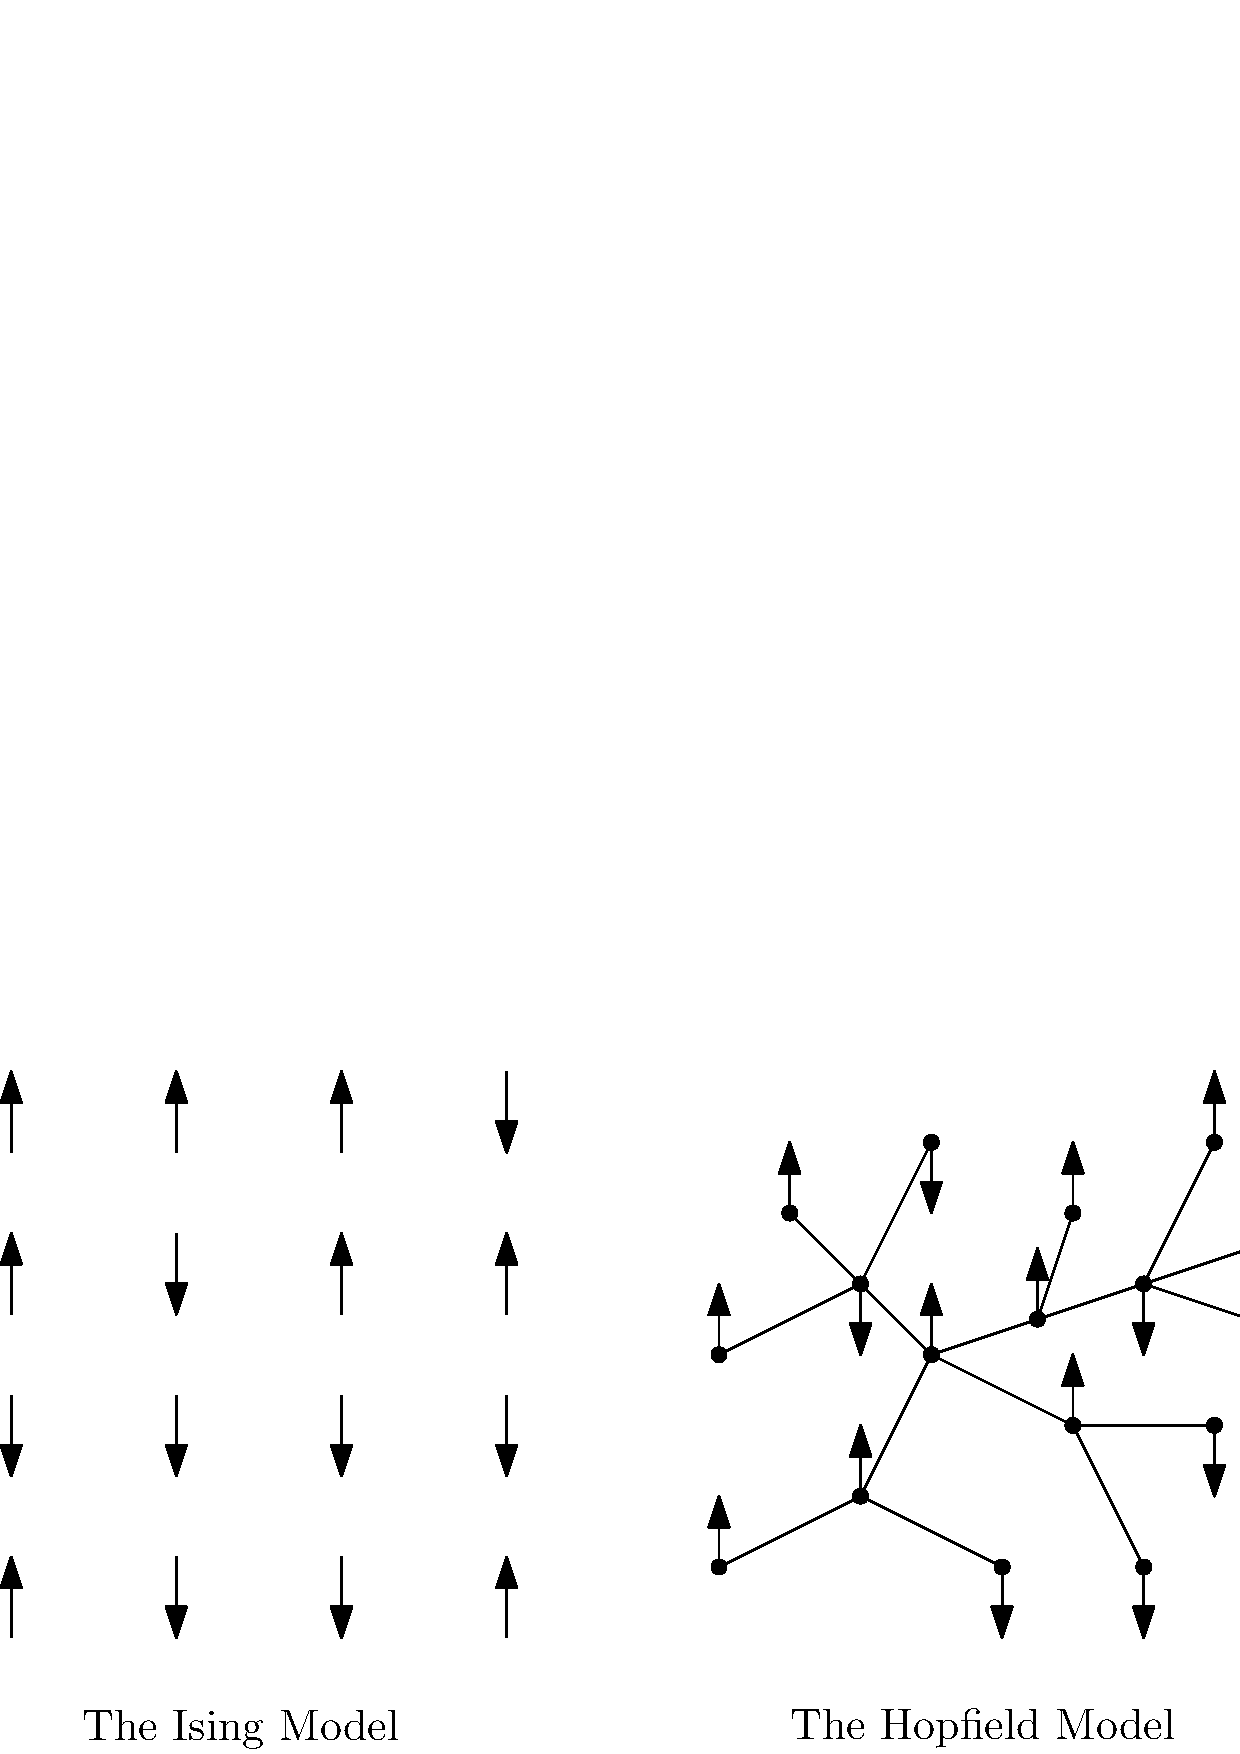
\includegraphics[width=\textwidth]{figures/evolution-anns.pdf}
  \caption{Restricted Boltzmann machines are a binary-valued two-layer
    neural network. RBMs trace their origins to the Hopfield model, an
    early model for associative memory which itself was inspired by
    the Ising model~\cite{hopfield}.\label{fig:rbm} }
\end{figure}

A full review of the techniques available in ML is beyond the scope of
this capstone. As such, we will focus our attention on one particular
class of algorithms, restricted Boltzmann machines (RBMs),
bidirectional artificial neural networks for modeling probability
distributions.  Depicted in \fref{fig:rbm}, RBMs consist of two layers
of binary units: a \textit{visible} layer,
${\bv}\eqcolon{\setv}_{i=0}^N$, and a \textit{hidden} layer,
$\bh\eqcolon\seth_{j=0}^N$, where $v_i,h_j\in\{0,1\}$. The visible
layer will serve as the input for our data, $\bx\rightarrow\bv$, and
the hidden layer as our prediction, $\bh\rightarrow\by$, the
label. For the purposes of classifying the phases of the 2D Ising
model, it will suffice to consider an RBM with one hidden unit,
$h$. If $h$ is $1$, we predict that the configuration is in the
ordered phase, and for $h=0$, we predict disordered. From our
exploration in the previous chapter, we could probably come up with
some function that performs this prediction. For example, we might sum
all of the spins (compute the magnetization), and if the result is
close to $0$ we know the system is disordered: $h:=0$. Otherwise, we would output $h\eqcolon 0$. The power of ML
will be to extract rules like these without explicit instructions.

Instead, we teach our model implicitly through the cost function,
$\mc{C}(P_{\theta}(y\rvert\bx), \{\mcX_{data}, \mcY_{data}\})$. This
acts as a moderator, and it tells the model how ``incorrect'' its
predictions (labels) are.  Formally, the ML goal becomes to find the
parameters $\theta$ that minimize $\mc{C}$. Experience from physics
tells us that finding the ground state (global minima) can be really,
\textit{really} hard.  Instead, we use stochastic gradient descent
(SGD). For each $\theta$, we calculate $\partial_{\theta}\mc{C}$, with
which we implement the update rule:
\begin{equation}%
  \theta \rightarrow \theta - \eta \partial_\theta \mc{C},
\end{equation}%
where $\eta$ is the \textit{learning rate}. From calculus, we know that the
negative gradient of a function is the direction in which that
function decreases most rapidly. This update procedure, then, adjusts
our parameters so as to reduce the cost. Iterating this procedure, we
end up in a local minimum of the cost function \sref{fig:sgd}. In
practice, we calculate these gradients, not over the entire data set,
but over subsets, \textit{minibatches}. This means the gradients will
vary from iteration to iteration (hence, \textit{stochastic}). This is
both computationally faster and introduces noise (like temperature)
that improves the chances of escaping poor local minima.

\begin{figure}[ht]
  \centering \includegraphics[width=0.75\textwidth]{figures/sgd.png}
  \caption{Stochastic Gradient Descent (SGD). If we view the cost
    function as defining an ``energy'' landscape, SGD allows us to
    find local minima (stable or metastable) energy states. Image
    taken from~\cite{sgd}.\label{fig:sgd} }
\end{figure}

Now, if we can formulate an adequate prediction function,
$P(\bh\rvert\bv)$, for the RBM, we can improve it with SGD. The
crucial step is to define an energy function:\label{sec:rbm-energy}%
\begin{equation}%
  \boxed{E_\theta(\bv, \bh)\eqcolon-\sum_i a_iv_i -\sum_j b_jh_j-\sum_{ij} w_{ij}v_ih_j \label{eq:rbm-energy-fn}}
\end{equation}
where $\theta\eqcolon\{\{a_i\},\{b_j\},\{w_{ij}\}\}$. Then, we can
model the system's joint probability with a Boltzmann distribution:%
\begin{equation}%
  \boxed{P_\theta(\bv,\bh)\eqcolon\frac{1}{Z}e^{-E_\theta(\bv,\bh)},\tab
    Z\eqcolon\sum_{\bv',\bh'}e^{E_\theta(\bv', \bh')}\label{eq:rbm-joint-dist}}
\end{equation}%
We note that this is the exact same equation as our Ising model
(\ref{eq:boltzmann-distribution} and~\ref{eq:ising-energy}). Here,
$\{a_i\}$ and $\{b_j\}$ take the role of the external magnetic field
$B$, which now varies from site to site (hence the indices $i$ and
$j$). Then, $\{w_{ij}\}$ takes the role of $J$ varying from pair to
pair.

Naturally, we run into the same intractability issues. For large
enough networks, we cannot evaluate $Z$. Instead of calculating joint
distributions, we pull a trick similar to MFT and MCMC, considering
instead conditional and marginal distributions. Due to RBM's bipartite
structure these factor and are easy to evaluate. Explicitly, in the
case of a single hidden spin $h_j$, we get (with a bit of algebra):
\begin{align}%
  P(h_j\rvert\bv)&=\frac{P(h_j,\bv)}{P(\bv)}=\frac{(e^{-E(\bv,h_j)})/Z}{(\sum_{\bh'}e^{-E(\bv,\bh')})/Z}\\
                 &=\frac{e^{-h_j(\sum_i w_{ij}v_i+b_j)}}{1+e^{(\sum_i w_{ij}v_i+b_j)}}.
\end{align}%
This conditional probability is itself a Boltzmann distribution, but
over only two states (tractable!).  We get for the full system:
\begin{equation}
  \boxed{P_\theta(\bh|\bv)=\prod_{j=1}^M \frac{1}{1+e^{-h_j(\sum_i w_{ij} v_i +b_j )}}
  }\label{eq:v-to-h}
\end{equation}%
and similarly:
\begin{equation}
  \boxed{P_\theta(\bv|\bh)=\prod_{i=1}^N \frac{1}{1+e^{-v_i(\sum_j w_{ij} h_j + a_i )}}
  }\label{eq:h-to-v}
\end{equation}

All that remains is for us to choose an adequate cost-function, and we
can start training our RBMs. For the example of binary-classification,
an appropriate choice is the cross-entropy loss:%
\begin{equation}%
  \mc{C}(P_\theta(\by\rvert\bx), \{\mcX_{data}, \mcY_{data}\})=\sum_{\bx\in\mcX_{data}} \sum_{\by\in\{0,1\}} P_{true}(\by\rvert\bx)\log P_\theta(\by\rvert\bx),
  \label{eq:cross-entropy}
\end{equation}%
see \sref{sec:cross-entropy} for elaboration. Differentiating with
respect to $\theta$ and with some simple algebra, we get the training
rule:%
\begin{align}%
  \partial_{b_j} \mc{C}&=\sum_{\bx\in\mcX_{batch}} P_{true}(\by\rvert\bx) \big[1-P_\theta(\by\rvert\bx)\big]\left(h_j\right),\\
  \partial_{w_{ij}}\mc{C}&=\sum_{\bx\in\mcX_{batch}} P_{true}(\by\rvert\bx)\big[1-P_\theta(\by\rvert\bx)\big]\left(v_i h_j\right).
\end{align}%
We have all the necessary elements of a phase classifier: a dataset, a
model of $P(\by\rvert\bx)$, and a means to train this model. In the
next section, we will consider an example more relevant to the
statistical physicist: generating samples.

\section{Generative Modeling: Gibbs
  Sampling}\label{sec:rbm-generative-modeling}
In \fref{sec:mc-overview}, we considered how to use MCMC sampling to
estimate macroparameters and even critical exponents.  Here we will
consider an MCMC technique called \textit{Gibbs Sampling} which will
use RBMs to generate samples of $P(\bx)$.

Suppose we are given an already trained RBM\@. Gibbs sampling, like other
MCMC techniques, consists of a series of update steps. In one step, we
input some initial state, transform it into a hidden state using
$P_\theta(\bh\rvert\bv)$, and transform it back to a new visible state
using $P_\theta(\bv\rvert\bh)$. This process is imperfect, so the
output of one step will differ from the input. If we repeat this
process many times, then the distribution of the outputs will converge
to the equilibrium distribution $P_\theta(\bv)$.

This first requires $P_\theta(\bv)$ to be an appropriate model of
$P_{true}(\bv)$. To get to this point, we need to derive a marginal
distribution over $\bv$ from $P_\theta(\bv,\bh)$. Similar to the
conditional probabilities, the architecture of the RBM allows us to
perform the marginalization
$P_\theta(\bv)=\sum_{\bh}P_\theta(\bv,\bh)$ explicitly. If we write
$P_\theta(\bv)$ as a Boltzmann distribution with its own energy
$E_\theta(\bv)$,
\begin{equation}%
  P_\theta(\bv)=\sum_{\bh} P_\theta(\bv,\bh) \propto e^{-E_\theta(\bv)},
\end{equation}%
then we can express $E_\theta(\bv)$ in terms of $E_\theta(\bv,\bh)$
\sref{sec:marginal}:
\begin{equation}
  \boxed{
    E_\theta(\bv)=-\sum_i a_i v_i -\sum_j \log\left(1 + \exp{-\left(b_j + \sum_{i} v_i w_{ij}\right)}\right),
    \label{eq:rbm-marginal-energy-v}
  }
\end{equation}
and we can perform an analogous computation for the marginal
distribution over $\bh$ to get $P_\theta(h)$ as a Boltzmann
distribution in terms of energy, $E_\theta(h)$. As in the
classification example, we require a cost function, in this case, the
Kullback-Leibler divergence (KLD):%
\begin{equation}
  \mc{C}(P_\theta(\bx),\bx)=D_{KL}(P_{data}(\bx)||P_{\theta}(\bx))\eqcolon\sum_{x\in\mcX_{data}} P_{true}(\bx)\ln\left(\frac{P_{true}(\bx)}{P_{\theta}(\bx)}\right). \label{eq:kld}
\end{equation}
This is closely related to the cross-entropy, and, similarly, it is an
important information-theoretic quantity \sref{sec:kld} that provides
a notion of similarity for probability distributions. It is $0$ if and
only if the two distributions are equal:
\begin{equation}%
  D_{KL}(P_{true}(\bx)||P_{\theta}(\bx))=0\iff P_{true}(\bx)=P_{\theta}(\bx).
\end{equation}%

We claimed that this unsupervised, but in comparing $\mc{C}$ in \fref{eq:kld}
with \fref{eq:cross-entropy}, we might interpret $\bx$ as a kind of
label for itself. A more appropriate description is
\textit{self-supervised}. We emphasize this point because it has been
the source of misunderstanding. ML always requires the specification
of a cost function, and even in the absence of labels, the cost function
guides how the model learns which information is relevant and irrelevant.

If we differentiate the KLD with respect to $\theta$, then after a bit
of algebra, we get:%
\begin{align}%
  \partial_{a_i} D_{KL}&=\expect{v_i}_{true}-\expect{v_i}_\theta\\
  \partial_{b_j} D_{KL}&=\expect{h_j}_{true}-\expect{h_j}_\theta\\
  \partial_{w_{ij}} D_{KL}&=\expect{v_i h_j}_{true}-\expect{v_i h_j}_\theta
\end{align}%
where $\expect{\ldots}_{true}$ is an average over the true
distribution $P_{true}(\bv)$ and $\expect{\ldots}_{\theta}$ is an
average over the model distribution $P_{\theta}(\bv)$.

If you take away one thing from this capstone, let it be this: sums
and averages like these are hard. Naturally, we approximate. Wherever
$h_j$ shows up, we use $P(h_j|\bv)$, and for the expectations over
$P_{true}$, we calculate a Monte Carlo average over our dataset,
$\mc{X}_{data}$. The expectations over $P_\theta$ are trickier. Fortunately,
we can approximate them with Gibbs sampling, initializing with samples
from $\mc{X}_{data}$. Together, these approximations constitute the
\textit{contrastive-divergence} algorithm, see~\cite{hinton}. Having trained our RBM, we
can generate new samples and start calculating critical exponents.

RBMs trained in this way have applications other than generation.
Consider training these on black and white images: if we constrain the
number of hidden nodes to be less than the number of visible nodes,
then the hidden layer will learn a compact representation of the
input. We can even stack multiple RBMs on top of each other to form
\textit{deep Boltzmann machines} (DBMs). In DBMs, the hidden layer of
one RBM becomes the visible layer of the next. Trained with
contrastive divergence, each layer learns a progressively compacter
version of the input.  This should remind you of RG\@. In the next
section, we will make these similarities more exact. Ultimately, this
allows us to machine learn RG transformations.


\chapter{Machine Learning and the Renormalization
  Group}\label{sec:comparison}
In the previous chapter, we considered two examples of ML in physical
investigations: neural networks used as a phase classifier and MCMC
sampler. Consider the superficial similarities between these neural
networks and our treatment of RG in \fref{sec:crit-phenomena}. The
classification example calls to mind the infinite RG limit in which
all disordered phases flow to one fixed point and all ordered phases
to another. Here, these fixed points would correspond to the values of
our label being either $0$ or $1$. The generative example is more
immediately similar, and the very language is analogous: we speak of
hidden layers that hierarchically decompose the input visible layer to
coarse-grained hidden layers. We might be tempted to ask: does a DBM
of, say, five layers learn to implement four iterations of some RG
procedure \sref{fig:rbm-rg}?

\begin{figure}[ht]
  \centering \includegraphics[width=0.5\textwidth]{figures/rg-rbm.png}
  \caption{Two iterations of block renormalization and a deep
    Boltzmann machine of three layers.\label{fig:rbm-rg} }
\end{figure}a


However, questions like this are too general. We have already seen two
examples of RBMs used for different goals, and what constituted relevant
information differed in either context. In RG, relevant information is
understood more narrowly: it is the long-distance information. If we
are to make comparisons between RG and RBMs, we must be more specific,
and this begins by being more precise in our definition of
``relevant'' information. Although Claude Shannon, the founder of
information theory, avoided this topic explicitly, Tishby et al.\
showed that information theory provides a natural and exact
formulation of relevant information: relevant information is simply
the information contained in one signal, $\bx$, about another
$\by$~\cite{tishby}. For our phase classifier, the relevant
information is the information contained in the Ising samples $\bx$
about the labels $\by$. Once we have trained RBMs for compression, the
relevant information is the information contained in the hidden layer
$\bh$ about the visible layer $\bv$. Information theory quantifies how
much information is shared between two signals with the mutual
information:
\begin{equation}%
  I(\bx; \by)\eqcolon\sum_{\bx,\by}P(\bx,\by)\log\left(\frac{P(\bx,\by)}{P(\bx)P(\by)}\right),\label{eq:mutual-info}
\end{equation}%
We see this quantity is minimized ($I(\bx;\by)=0$) when the random
variables are independent ($P(\bx,\by)=P(\bx)P(\by)$). It is maximized
when the variables are maximally dependent. We have a quantitatively
basis for extracting relevant information: maximizing mutual
information between appropriately chosen signals.

In the next chapter, we will derive the correct choice for $\bx$ and
$\by$ on lattice systems that recovers physically-relevant (i.e.\
long-distance) information. We then derive a variational proxy to the
mutual information that we can differentate and, thus, learn in a
neural network.

With the knowledge of an exact formulation of relevant information, we
can start investigating links between particular RG implementations
and RBMs. Such comparisons will revolve around the question of
relevance. What information does a given cost-function deem relevant?
Are there examples where this overlaps with our notions of physical
relevance? Let us consider a seminal example.

\section{A Comment on Mehta and Schwab's Equivalence}
As a first attempt, we will consider Mehta and Schwab's correspondence
between Kadanoff's variational procedure \pref{sec:kadanoff} with RBMs
trained by contrastive divergence
\pref{sec:rbm-generative-modeling}~\cite{mehta}. Specifically, we
consider the narrower case, of ``exact'' RG and ``exact'' RBMs. Exact
RG means that Kadanoff's transformation preserves \textit{all} the
information contained in the hidden system; i.e.\ the free energy of
the input and coarse-grained systems is exactly the same. Similarly,
an exact RBM has learnt to perfectly recreate its inputs
$P_{true}(\bx)=P_\theta(\bx)$ in \fref{eq:kld}; the RBM will have
reached a global minimum of the cost function.

First, Mehta and Schwab show that, under the above conditions, the two
transformations are equivalent under:%
\begin{equation}
  \bT_\theta(\bv, \bh)=-\bolds{E}_\theta(\bv,\bh)+\bolds{H}(\bv),
\end{equation}
and we provide the derivation in \fref{sec:mehta-equivalence}.

However, the exact case is not generally possible, and when it is, it
is often not particularly interesting. Exact RBM transformations
likely mean overfitting which is likely opposed to the aims of the ML
investigation. Exact RG transformations are few and far between, so
this correspondence would apply only under narrow circumstances. More
interesting then, would be to consider a non-exact comparison.

Here, the two approaches will vary: Kadanoff's variational method
operates at the level of free energies while contrastive divergence
works at the level of probabilities, and optimizations at these
different levels will not necessarily coincide. Still, there may still
be qualitative similarities. Pursuing this line of inquiry, Mehta and
Schwab train RBMs as described in
\fref{sec:rbm-generative-modeling}. They find that the RBMs learn to
couple hidden units to local blocks of visible units.\footnote{
  Crucially, this was not possible without \textit{regularization}, a
  technique that promotes sparse connections, between hidden and
  visible units see~\cite{mehta-review}.}
\begin{figure}[ht]
  \centering \includegraphics[width=0.5\textwidth]{figures/mehta.png}
  \caption{Visualization of the receptive filters of the hidden units
    in one of the layers of the DBM trained by Mehta and
    Schwab~\cite{mehta}. Each plot corresponds to one hidden unit, and
    each pixel corresponds to one spin in the initial layer. Higher
    intensities mean the hidden unit is more coupled to that
    spin. Indeed, we see that the RBM learns to couple local
    transformations. However, the transformations do not preserve
    nearest neighbor relations. This does not matter for the total
    amount of information stored in coarse-grained layers. In RG,
    these concerns do matter because they affect the practicality and
    interpretability of result~\cite{kjr}.\label{fig:fig:mehta} }
\end{figure}

Mehta and Schwab write:%
\begin{quote} Surprisingly, this local block spin structure emerges
  from the training process, suggesting the [deep neural network] is
  self-organizing to implement block spin
  renormalization~\cite{mehta}. % write out DNN somewhere.
\end{quote}

These RBMs may indeed learn a kind of block-spin
transformation. However, this block-spin transformation need not be
block-spin \textit{renormalization}. As Koch-Janusz and Ringel put it:
\begin{quote}
  [T]he usefulness (and practicality) of the RG procedure depends on
  choosing [the transformation] \ldots such that the effective
  Hamiltonian\ldots remains as short range as possible.~\cite{kjr}
\end{quote}
More precisely, in the Taylor expansion of our coarse-grain
Hamiltonians, the shortest range terms should dominate:
\begin{equation}%
  H(\bs)=-\sum_i K^{(1)}_{i} s_i - \sum_{\expect{i,j}}K^{(2)}_{ij}s_i s_j-\sum_{\expect{\expect{i,j}}}K^{(3)}_{ij}s_i s_j\ldots,
\end{equation}%
with $K^{(n)}$ are exponentially suppressed in $n$. In RG, we place
additional constraints on how to organize the information in
subsequent layers. Block renormalization procedures, including
Kadanoff's technique, respect the symmetries and topology of the
system under consideration. The locality of interactions means
neighboring visible blocks of spins become neighboring hidden
spins. Translational symmetry means the same transformation is applied
to each block.  Mehta and Schwab's RBMs will not, in general, satisfy
these two conditions.

Let us be more exact, rephrasing renormalization in probabilistic
terms: we parametrize our RG transformation as the conditional
probability distribution $P(\bh\rvert\bx)$, where $\bx$ is our initial
configuration and $\bh$ is the hidden or coarse-grained
configuration. Locality and translational invariance of the Ising
model mean we can factor the RG transformation into a product of local
single-block transformations. We divide the system into $M$ blocks,
$\bx\rightarrow\{v^{(1)}, v^{(2)},\ldots, v^{(M)}\}$, with
corresponding hidden units $\{h_1, h_2,\ldots,h_M\}$. Then we can
factor $P(\bh\rvert \bx)$ as:
\begin{equation}%
  P(\bh\rvert\bx)=\prod_{j=1}^M P(h_j\rvert \bv^{(j)}).\label{eq:prob-block-rg}
\end{equation}%
Consider what happens, when you permute the units in the hidden layer;
i.e., we use a different transformation $P(h_{j'}\rvert \bv^{(j)})$
where $j\neq j'$.  As long as our reverse rule, $P(\bx\rvert\bh)$ also
takes this into account, such a permutation has no impact on the
performance of Mehta and Schwab's contrastive divergence trained
RBMs. This is \textit{not} the case in RG\@. There is a unique
permutation of hidden layer degrees of freedom which maximizes the
above short range condition, and acceptable RG transformations
identify this permutation.

Furthermore, the block transformations that the RBM learns may not be
the same for each block. Compression and generation are invariant
under partial flips $h_j:(0,1)\rightarrow(1,0)$, for some fixed
$j$.\footnote{RG transformations are invariant under a collective flip
  of $\bh$.} Blocks of spins which were perfectly correlated in the
visible layer may be perfectly anticorrelated in the hidden
layer. Although the information content is the same, the hidden layer
Hamiltonian will take a more complicated form than is necessary, going
against notions of what is a good and practical RG procedure.

Mehta and Schwab fail to mention these conditions, so their suggestion
that RBMs learn block-spin renormalization falls short. However, if we
make these conditions explicit, we can easily recover a stronger
version of their claim. To do this, we introduce convolutional neural
networks (CNNs) as depicted in \fref{fig:cnn}. These are networks with
a special architecture: instead of all-to-all couplings, we explicitly
couple spins in the hidden layer to blocks in the visible
layer. Additionally, CNNs perform the same translation for each block
and respect the topology of the input system. Had they required a
convolutional architecture upfront, Mehta and Schwab may, indeed, have
successfully trained RBMs to learn even block renormalization.


\begin{figure}[]
  \centering \includegraphics[width=\textwidth]{figures/cnn.png}
  \caption{This is LeNet-5, an example of a convolutional neural
    network used for digit recognition and a seminal
    architecture~\cite{lecun}.\label{fig:cnn} }
\end{figure}

From these observations, we can make the link between majority-rule
block-spin RG and ML fully precise.  In \fref{sec:majority-rule-rbm}, we
derive a equivalence between RBMs an RG, describing a parameterization
which implements the majority-rule:
$P(h_j|\bv^{(j)})=\sgn \sum_i v_i^{(j)}$.

\section{Relevant Information}
For the exact case discussed by Mehta and Schwab, we preserve the full
probability measure which necessarily preserves the long-distance
information. However, in the non-exact case, the KLD has no preference
for long-distance information over short-distance: all information is
valued equally. In the case of compression and generation, this is
acceptable: we have no a priori knowledge of which features in the
data are more important.

In RG, we have stronger requirements: transformations must favor
long-distance information over short-distance information. We can say
resolutely: RBMs trained with the KLD (even with the appropriate
convolutional architecture) need not learn acceptable RG
transformations. Perhaps in the case of the simple Ising model, the
KLD is an adequate heuristic. However, we have no guarantee that this
extends to novel systems. In fact, Koch-Janusz and Ringel showed that
RBMs trained with the KLD on the dimer model, another model from
statistical physics, couple to local fluctuations rather than to the
correct hidden variables~\cite{kjr}. We recall that appropriate
transformations for one system need not translate to others
\sref{sec:kadanoff}. Critique of Mehta and Schwab's paper revolves
primarily around the KLD being an inappropriate criterion for RG
transformations~\cite{lin, iso}.

In reply, Mehta and Schwab point out that Kadanoff's method also
offers no guarantee of extracting the correct physical information. We
come back to the difficulty of devising appropriate RG techniques, and
the need for creativity. In fact, this need for intuition in RG is
mirrored quite clearly in ML\@. Decisions regarding model
architectures and cost functions require creativity on the part of the
researcher. Both fields would benefit from a clearer understanding of
when techniques will and will not work. In the next chapter, we will
see that information theory may provide the framework to answer
questions like these, and we will encounter a system-independent
formulation of RG\@. This might mean better, more efficient models in
both disciplines.


% SECTION 4: RSMI ALGORITHM
\chapter{Renormalization in Information Theory}\label{sec:rsmi}
In the previous chapter, we used information theory to formalize the
notion of \textit{relevant} information. In this chapter, we will
adapt this to our physical context of long-distance as relevant
information. Ultimately, this allows us to devise a cost-function that
measures the physical information. From this, we can derive a learning
rule to train RBMs to perform \textit{optimal} transformations.

In the previous chapter, we saw that the Ising model's locality and
translational invariance conditions reduce the number of acceptable RG
procedures. Rather than devise an update rule for how an entire
configuration should transform under RG, we can start with
\fref{eq:prob-block-rg}.  Then, we only need to learn the
transformation for a single block, $P(h_j\rvert \bv^{(j)})$. We
already know that we can model conditional probabilities like these
with RBMs. This is the first insight of Koch-Janusz and Ringel, and in
this chapter, we will follow their information-theoretic
treatment~\cite{kjr}.

\section{An Information-Theoretic Formulation of RG}
First, we partition a full lattice configuration $\bx$ into four
areas: a visible block, $\bv$, that is surrounded by, in order, a
buffer, $\bb$, an environment, $\be$, and an outer area, $\bo$
\sref{fig:rsmi-overview}. In RG, we introduce a hidden area,
$\bh\eqcolon\{h_i\}$ which is a function of the degrees of freedom in
$\bv$. Our aim is to choose this coupling, $P(\bh\rvert\bv)$, so that
$\bh$ encodes the long-distance degrees of freedom about our system at
large, $\bx$\footnote{We have dropped the indices for convenience, and
  now we let block $\bh$ consist of multiple coarse-grained
  spins.}. By our assumption that $\bo$ is farther than the
correlation length, $\bv$ contains no information about $\bo$. We can
ignore $\bo$ in devising $P(\bh\rvert\bv)$. Furthermore, in coming up
with a function for $\bh$, we can reasonably ignore $\bb$. The
information contained in $\bv$ about $\bb$ is likely to be
short-range. By eliminating $\bb$, we throw out the shortest-range
fluctuations.
\begin{figure}[ht]
  \centering \includegraphics[width=0.5\textwidth]{figures/kjr.png}
  \caption{The RSMI algorithm partitions configurations into four
    regions, a visible block $\bv$, buffer zone $\bb$, environment
    $\be$ and outer zone, $\bo$. We introduce a coarse-grained block
    of spins $\bh$.\label{fig:rsmi-overview} }
\end{figure}%
That which remains is the physically relevant information; we see it
is the information shared between $\bv$ and $\be$. Our goal is to
extract this information and encode in $\bh$. We choose the
parameters, $\L$, of our RBM that models $P(\bh\rvert\bv)$ to maximize
the mutual information between $\bh$ and $\be$:%
\begin{equation}%
  I(\bh; \be)=\sum_{\bh,\be}P(\bh,\be)\log\left(\frac{P(\bh,\be)}{P(\bh)P(\be)}\right),\label{eq:rsmi}
\end{equation}%
where these probabilities are defined as marginalizations over
$P(\bx)$:%
\begin{align}%
  P(\bh, \be)&=\sum_{\bv}P(\bh\rvert \bv)P(\bv,\be)\\
  P(\bh)&=\sum_{\bv,\be}P(\bh\rvert \bv)P(\bv,\be)\\
  P(\bv,\be)&=\sum_{\bb,\bo}P(\bx)\\
  P(\be)&=\sum_{\bb,\bv,\bo}P(\bx).
\end{align}%

From previous chapters, we know that the probability measure $P(\bx)$
and its marginalizations are generally intractable. The key insight of
Koch-Janusz and Ringel is that we can use RBMs not only to model
$P(\bh\rvert \bv)$ but also to model these other
distributions. Koch-Janusz and Ringel ultimately use three RBMs: one
for $P(\bv,\be)$, another for $P(\bv)$, and finally the
$P(\bh\rvert\bv)$ RBM already mentioned. The other distributions are
calculated as MC-averages over the dataset. Hereby, Koch-Janusz and
Ringel derive a proxy to the mutual information \sref{sec:rsmi-calc}
which they can optimize with stochastic gradient descent.

To validate their ideas, they provide both experimental and
theoretical justification. For the 1D Ising model, these
marginalizations can be calculated exactly, and they show that
maximizing the RSMI rederives decimation, an RG procedure known to be
\textit{optimal} for the 1D Ising model in that the procedure does not
increase the range of the coarse-grained Hamiltonian.  In follow-up
research, Lenggenhager et al. (along with the aforementioned authors)
show that RSMI coarse-graining is more generally optimal, maintaining
short-distance in any number of dimensions. They further show this
holds even in some cases that the mutual information is not fully
saturated.  We direct the interested reader to~\cite{kjr}
and~\cite{lenggenhager} for these results.  In the remainder of this
capstone, we discuss our own implementation and generalization.

\paragraph{Measuring Critical Exponents}
Having trained an RBM according to the RSMI algorithm, we can use
finite-size scaling \sref{sec:finite-size-scaling} to estimate,
finally, critical exponents. An important detail will be to devise a
``thermometer'' that can measure the effective temperature at
successive RG-iterations. We discuss several options in
\fref{sec:thermometer}. These options, moreover, are intrinsic and do
not require explicit knowledge of the temperature. This means the RSMI
algorithm is fully unsupervised. If we encounter new systems where we
do not know the proper RG transformations (or even how to measure
``temperature''), then unsupervised approaches might save us
considerable headache. Rather than guess and check possible
transformations, we would first machine learn a renormalization
procedure on the system, then, observe and interpret, only later
attempting more calculation-heavy approaches. As Koch-Janusz and
Ringel put it, the RSMI algorithm could form the basis of the
``physical reasoning process'' itself~\cite{kjr]}. Instead of retroactively
explaining trends in our data, ML would proactively guide our
exploration.


% SECTION 5: VALIDATION OF RSMI ALGORITHM & EXTENSION
\chapter{Results: Machine Learning Critical Exponents}\label{sec:validation}
In~\cite{rgpy}, we release \textit{rgpy}, an open-source library for
implementing ML-based renormalization group techniques. This is still
in its infancy, and development is ongoing. As of now, it contains a
full-stack realization of the RSMI algorithm implemented in
Tensorflow: i.e., the package includes implementations of various MCMC
techniques (Metropolis-Hastings, Swendsen-Wang, and Wolff algorithms),
the RBMs necessary for the RSMI algorithm, and an implementation of
standard block-spin renormalization. We also provide a host of
already-generated samples at various lattice sizes and
temperatures. We invite the reader to explore and try out these tools.

\section{A Novel Calculation of $\bolds{\nu}$ for the 2D Ising Model}
Our exploration of statistical physics and ML was centered around the
Ising model and its macroparameters and critical exponents. The
calculation of these exponents served as unifying thread, and as
validation of the RSMI algorithm, we provide the following approximation
of $\nu$:
\begin{equation}%
  \boxed{\nu\approx 0.79 \pm0.39}
\end{equation}%
For how we calculated this, see
\fref{sec:methods}. This is not, by any means, an improved calculation.
However, it is a highly promising first result. The quality of this
calculation was ultimately limited by both time and hardware
constraints. With more of both, the prediction should eventually
converge to the right quantity.
\begin{figure}
  \centering
  \includegraphics[width=0.75\textwidth]{figures/crit-exponent.png}
  \caption{The finite-size scaling curve for the correlation length
    critical exponent.\label{fig:nu} }
\end{figure}
In fact, this result is just the start. Our investigation revealed a
large number of possible improvements and generalizations. Due to the
time contraints of this capstone, we have not yet implemented these
ideas, but, all the same, these ideas merit attention. The
generalization we discuss gives rise to a family of RSMI-inspired
techniques, together constituting a new branch of RG methods.

\section{A Generalization to $n$-Spin and $O(n)$ Systems}
Koch-Janusz and Ringel claim the RSMI algorithm works for general
lattice systems.  However, the current formulation works only for
systems with binary degrees of freedom: spin-$1/2$ Ising models. The
authors avoid explicitly generalizing these results.  Though the
generalization is straightforward, it is important enough to warrant
elaboration.

Let us consider systems with either $n$ spins or $n$ components of spin, then, the visible
units of our RBM should be able to take $n$ values. Accomplishing this
is quite simple: we let our visible units become vectors with $n$
components: $v_i\rightarrow \{v_{id}\}_{d=1}^n$.  We say that $v_i$
takes the value of spin $d$ when:
\begin{equation}%
  v_i \equiv d \iff
  \begin{cases}
    v_{id}=1\\
    v_{id'}=0, d'\neq d.
  \end{cases}
\end{equation}%
In fact, we will use the RBM to model a slightly different vector:
\begin{equation}%
  v_{id}=P(d),
\end{equation}%
where the vector is normalized $\sum_d v_{id}=1$. Such a vector that contains
probabilities of classes is called a \textit{one-hot
encoding}, and with these probabilities, we can randomly sample values
of spin to generate $n$-valued spins. For $n$-vector models, we leave
the probabilities as they are. To allow our RBMs to produce these
encoding, we have to introduce the index $d$ in the parameters of our
model:
\begin{align}%
  a_i &\rightarrow a_{id}\\
  w_{ij}&\rightarrow w_{ijd}.
\end{align}%
To derive a one-hot encoding, we change the RBM's reverse update rule,
$P(\bv\rvert \bh)$ (\ref{eq:h-to-v}).  The conditional probabilities
will still factor, but normalization over the scalar values $v_i=0,1$,
becomes normalization over the components of the vector, $d$.  If we
denote $\epsilon_i \eqcolon -(\sum_j w_{ij} h_j + a_i )$, then, whereas
before, we had:%
\begin{equation}%
  P(v_i\rvert\bh)=\frac{e^{-\epsilon_i v_i}}{\sum_{v_i'\in\{0,1\}} e^{-\epsilon_i v_i'}},
\end{equation}%
now we have, $\epsilon_{id}\eqcolon-(\sum_j w_{ijd}h_j+ a_{id})$, so:
\begin{equation}%
  P(v_{id}\rvert\bh)=\frac{e^{-\epsilon_{id} v_{id}}}{\sum_{d=1}^n e^{-\epsilon_{id} v_{id}'}}.
\end{equation}%
For $n=2$, we rederive the previous rule with a suitable choice in
$w_{id}$, $a_{id}$. For reasonable values of $d$ (anything we might
encounter in practice), we can perform these calculations
explicitly. If we apply this change to each of the RBMs in the RSMI
algorithm, we will be able to model $n$-spin and $O(n)$
models. Note that since we did nothing to the hidden variables, these
will still be either binary or Bernoulli-valued. If we require that
the hidden spins take the same form as the input variables, as we
might demand with RG, then we also need to apply a completely
analogous change to the hidden unit of the $P(h_j\rvert \bv^{(j)})$
RBM, and we can apply the RSMI algorithm to generic lattice systems.

There is, in fact, more room for generalization. Consider an arbitrary
Hamiltonian for a system with binary-valued data $H(\bx)$. If we
Taylor expand this function, we would get:%
\begin{equation}%
  H(\bx)= a + \sum_i b_i x_i + \sum_{ij}c_{ij} x_i x_j.
\end{equation}%
These are \textit{all} the terms in the expansion.\footnote{For $p>1$,
  $x_i^p = 0$ or $1$.}  Then, barring the bipartite structure, the RBM
energy function already has the most general form we could possibly
consider.  However, when we make the switch to continuous or $n$-ary
valued data, this is no longer true: the Taylor-expansions become
infinite. In these cases, we might consider energy functions with
different, possibly higher-order interactions.  As long as we maintain
the bipartite structure, we can ensured that conditional probabilities
factor. Then, we can use variants of contrastive-divergence to
efficiently train these models. We need not even require that
$P(\bv\rvert\bh)$ and $P(\bh\rvert\bv)$ take the same form.  The first
might be Gaussian and the second a gamma distribution. Formally, we
can consider the extension of RBMs into the \textit{exponential
  family}, and for a full discussion of the possibilities, we refer
the reader to~\cite{welling}.  Suffice to say, there are more powerful
options for modeling probability distributions. Though the current
choices suffice for the spin-$1/2$ Ising model, these extensions may
prove necessary in investigating more complicated systems.

For all the exact results of Koch-Janusz and Ringel, their practical
implementation uses a proxy which does not fully capture the above
mutual information~\cite{kjr}. Here we see two possibilities. First, we can
improve Koch-Janusz and Ringel's approximation. The authors use a
cumulant expansion
\begin{equation}%
  \expect{\exp\{K(\bx)\}}=e^{\sum_{\k=0}^\infty\frac{1}{\k!} C_{\k}},
\end{equation}%
with cumulants expressed in terms of the moments
\begin{align}%
  C_1&=\expect{K},\\
  C_2&=\expect{K^2}-\expect{K}^2,\\
  C_3&=\expect{K^3}-3\expect{K^2}\expect{K}+2\expect{K}^3,\\
\end{align}%
and so on. In deriving the proxy, only the first term is kept
\sref{sec:rsmi-calc}. For better results, a first improvement could be
made by introducing additional terms.\footnote{We may even be able to
  avoid this expansion altogether, see \fref{sec:rsmi-calc}.} Second,
we can consider other approximations of the mutual information, and we
draw the reader's attention to a sampling of options in the
literature: contrastive predictive coding~\cite{oord}, Deep
InfoMax~\cite{hjelm}, and Mutual Information Neural
Estimation~\cite{belghazi}. All three examples use mutual information
as the basis for powerful unsupervised techniques. Though we avoid
details, similarities (and differences) with the RSMI algorithm
warrant further investigation.

Perhaps the most exciting future course of action is extending these
ideas to momentum-space renormalization. Rather than focus on lattice
models, our goal would be to solve quantum field theories. A first
attempt might use the quantum-to-classical mapping of the path
integral formalism~\cite{kjr}. More powerful however would be to use
the same physical and information-theoretic arguments to devise
conditions equivalent to \fref{eq:rsmi} from first fundamentals.


% SECTION 6: DISCUSSION
\chapter{Discussion and Conclusions}\label{sec:discussion}
Let us summarize what we have accomplished.  We began overviewing the
basic elements of statistical physics which has the goal of turning
microscopic theories into concrete macroscopic observables.  One
quickly runs into a problem: intractable probabilites.  We sampled a
host of techniques that sidestep this fundamental problem. MCMC
techniques avoid absolute probabilities with iterations of relative
probabilities. Mean field theory uses a clever constraint on
conditional distributions. RG creates new probability distributions,
iteratively simpler, keeping the relevant long-distance information.
After an introduction to ML, we noticed a resemblance between neural
networks and RG\@. We identified a need for a more precise notion of
``relevant'' information, which one formalizes with information
theory. At the level of ``relevant'' information, ML and RG appeared
to behave similarly, extracting relevant information and suppressing
irrelevant information. However, we saw that RG contained a more
narrow conception of relevance: long-distance.

We evaluated Mehta and Schwab's seminal comparison of Kadanoff's RG
and CD-trained RBMs. We identified a flaw in one of their claims: a
``good'' RG, should uncover compact, short-range hidden
representations and respect the original system's symmetries, and RBMs
do not necessarily favor these unless explicitly told to. By being
more exact in formulating conditions, requiring convolution archictures,
we derived an exact correspondence between majority-rule
block-spin renormalization and restricted Boltzmann machines.

Using the information-theoretic formulation of relevance, one can
derive a system-independent RG criterion that \textit{optimally}
satisfies the short-distance condition. We implemented these ideas in
\textit{rgpy}, performing a recalculation of the critical length
correlation exponent. This library is available to everyone, and we
will continue developing it into the future. We encourage the reader
to try this out, and we hope to enable many more calculations of
critical exponents.  To kickstart this project, we provided an
overview of possible improvements and generalizations: the next likely
targets are the XY-model and the spin-1 Ising model.

We place special emphasis on the role physical reasoning played
throughout our exploration. Though information theory presented us a
formal notion of relevant information, it was physical reasoning that
led us to an appropriate RG condition. By explicitly thinking about
the properties physical systems possess, such as locality and
translational invariance, we managed to peak deeper into ``black box''
neural networks than may otherwise have been possible. We quote
Koch-Janusz and Ringel, ``the internal data representations discovered
by suitably designed algorithms are not just technical means to an
end, but instead are a clear reflection of the underlying structure of
the physical system''~\cite{kjr}. Integrating physical and ML
perspectives proves a promising basis for a better insight into these
algorithms.  Not to mention, these techniques are unsupervised, so
they should translate readily to problems other than the Ising model.

Comparisons and integrations of ML and RG are at an early phase, and
there remains much to be uncovered. It seems that information theory
is the appropriate framework with which to lay these links. Within
physics, a better understanding of this area may guide research into
new systems (on disordered, glassy systems and quantum field
theories), though the ramifications extend much
further~\cite{kjr}. Ultimately, the synthesis of ML, physics, and
information theory may teach us a thing or two about why these
techniques work as well as they do. Until then, the links should
inspire powerful new techniques in both of these disciplines.


\section*{Acknowledgements}
I would like to thank Marcos Crichigno for supervising this
capstone. I do not think either of us knew what we were getting into
when I first approached him, and I am stunned at how much I have been
able to learn during this time. Marcos provided guidance, much-needed
prodding, and a watchful eye, keeping the focus on the big
picture. The topics were new to both of us, ML for him and RG for me,
and getting to integrate these different perspectives was a wonderful
experience. I would also like to thank my dad, Jiri Hoogland, for
helpful feedback on drafts and, most of all, for his expertise on on
all things Monte Carlo. After being stuck with implementation details
of the RSMI algorithm for two weeks, his words finally let the penny
drop. As a last note, I would like to thank my friends and (other)
family for putting up with me during the last weeks (when I was a
little less than sociable), in particular, Nick van der Woude, for
mutually infectious enthusiasm.


% APPENDIX
0A\appendix
\chapter{Basics of Statistical Physics}
The proceeding derivations follow Cardy~\cite{cardy} and Domb~\cite{domb}.
\section{Measurements as Averages}\label{sec:measurements-as-averages}
Suppose we want to test whether our theory, the Ising model, lines up
with experimental results: what are the kinds of predictions we can
make? Our first attempt might be to measure the system's
magnetization, rather appropriate as this is the defining
characteristic of ``magnets.'' Before we do, however, let us be more
precise. What is a measurement, specifically for magnetization? The
magnetization, $M$, of any one microstate, $\bs$ is simply the sum of
the orientations of all spins, $s_i\in\bs$ in a given state:%
\begin{equation}%
  M(\bs)=\sum_{i} s_i,
  \label{eq:magnetization}
\end{equation}%

Generally, the microscopic state of a system is changing rapidly, and
the system will explore many different microstates over human
time-scales. Our measuring devices have finite resolution in time, so,
in a laboratory, we cannot perform sums over individual microstates. A
measurement becomes the average over the microstates visited during
the measurement period, weighted by the time spent in each state. In
statistical physics, we often work in the limit that the update time
goes to zero compared to the time of measurement. In this light, the
notion of a probability of a microstate is also the fraction of time
the system spends in that microstate over an infinite duration. Our
measurement outcome, $\mc{M}$, is an expectation value,
$\expect{M(\bs)}$, the average over the set of all microstates,
$\mcS=\{\bs\}$, weighted by the amount of time spent in each state,
$P(s)$:%p
% TODO: BETTER NOTATION (\bs conflicts with E(\bs)
\begin{equation}%
  \mc{M}=\expect{M(\bs)}=\sum_{\bs\in\{\bs\}}P(\bs)M(\bs).
  \label{eq:magnetization-expectation}
\end{equation}%
The same holds for any measurable quantity. Given some function of a
microstate, $A(\bs)$, the macroscopic value it corresponds to is its
expectation value over all microstates, $\expect{A(\bs)}$. Common
examples (not restricted to the Ising model) include $E(\bs)$, the
energy, $P(\bs)$, the pressure, and $V(\bs)$, the volume. If we can
find a probability measure over microstates, we can use the above to
calculate any macroparameter we choose.

\section{Thermal Equilibrium and the Second Law of
  Thermodynamics}\label{sec:delta-s-delta-e}
Consider the first law of thermodynamics (differential form with only
one kind of particle):%
\begin{equation}%
  dE=TdS-PdV+\mu dN,
\end{equation}%
where $E$ is the energy, $T$ the temperature, $P$ the pressure, $V$
the volume, $\mu$ the chemical potential, and $N$ the number of
particles.

For the canonical ensemble (our example), $dV$ and $dN$ are $0$.
Then, this reduces to:
\begin{equation}%
  \frac{1}{T}dE=dS.
\end{equation}%

From \fref{eq:boltzmann-entropy-difference}, we have
$\Delta S=S_{\br}(\bs)-S_{\br}(\bs')$.  If the reservoir is much
larger than $\bs$, this is a tiny difference, so
$\Delta S \approx dS$.  Then, we get
$\Delta S \approx \frac{1}{T}(dE)$. Note that this requires the
reservoir and system to have the same temperature (i.e., to be in
thermal equilibrium, $T_{\br}=T_{\bs}$).  We can use the same
approximation to expand this out:
$dE\approx E_{\br}(\bs)-E_{\br}(\bs')=\Delta E$.  We end up
with~\fref{eq:boltzmann-energy-difference}.

Note that in the thermodynamic limit,
$\abs{\bs}, \abs{br}\rightarrow \infty$ while maintaining the
inequality $1\ll\abs{\bs}\ll\abs{\br}$, these statements are precise
(this is simply the central limit theorem).

\section{Observables as Derivatives of the Partition
  Function}\label{sec:Z-to-macros}
Let us define the free energy, $F=-\frac{1}{\b}\ln Z$, where $\b=k T$,
the so-called thermodynamic beta. Consider an energy function with a
dependence on parameter $A$ according to:%
\begin{equation}%
  E(\bs)=E_0(\bs)+\l A(\bs)
\end{equation}%

Then, $\expect{A}=\partial_\l F$ The derivation proceeds as:
\begin{align}%
  \expect{A(\bs)}&=\partial_\l \left( -\frac{1}{\b}\ln Z\right) \label{eq:expectation-as-derivative}\\
                 &=-\frac{1}{\b Z}\partial_\l Z\\
                 &=-\frac{1}{\b Z}\sum_{\bs} e^{-\b E(\bs)}\partial_\l\left(-\b E(\bs)\right) \\
                 &= \frac{1}{\b Z}\sum_{\bs} e^{-\b E(\bs)}\left(\b A(\bs) \right) \\
                 &= \sum_{\bs} \frac{e^{-\b E(\bs)}}{Z} A(\bs) \\
                 &= \sum_{\bs} P(\bs) A(\bs).
\end{align}%

Consider an example, taking the Ising Hamiltonian
(\ref{eq:ising-energy}):
\begin{align}%
  \partial_B \left(-\log Z\right)&=-\frac{1}{Z}\sum_{\bs}\partial_Be^{-B \sum_i s_i - J \sum_{\expect{i,j}} s_i s_j}\\
                                 &=-\sum_{\bs}\frac{e^{-E(\bs)}}{Z} (-\sum_i s_i)\\
                                 &=\sum_{\bs}P(\bs)M(\bs) \\
                                 &=\expect{M(\bs)}.\label{eq:magnetization-as-derivative}
\end{align}%

Two others:
\begin{align}%
  \chi&=\partial_B \mc{M}=\partial_B^2F\\
  E&=\partial_\b F.
\end{align}

\chapter{Scaling and Renormalization}
\section{Finite-Size Scaling Analysis}\label{sec:finite-size-scaling}\
This section follows~\cite{fssa}. In our theoretic discussion, we have typically considered infinite
lattices: for a fixed lattice size $L$, we have let the microscopic
size $a$ (the lattice width) go to zero. Then, the dimensionless
$N=L/a$ (the number of lattice sites in a given dimension) diverges;
this is the classical thermodynamic limit.  Of course, truly physical
systems are finite with correspondingly non-singular partition
functions. For any such systems, there can be no divergences. An
important concern is, then, determining under which conditions we can
treat our systems as infinite and under which conditions finite-size
effects have a non-neglibile effect.

An important tool we use to study critical systems is MCMC
simulations: here, we quickly run into computational limits on the
sizes of lattices we can simulate. Especially for MCMC techniques, the
role of finite-size scaling is crucial.

Consider a $d$-dimensional Ising model infinite in all directions. If
we were to decrease $N$ of one dimension to some finite value, the
system's critical behavior begins to be dominated by a $d-1$
dimensional critical point. This is an example of crossing-over
behavior. By controlling some relevant parameter we change the
effective dimensionality of our system and navigate between different
critical points.

An example of this finite-size behavior is that of the correlation
length, $\xi$. It will no longer diverge and depending on the boundary
conditions will experience a peak at either above or below the infinte
critical point. For cyclical boundary conditions, the effective
critical temperature will increase, as the system is more ordered with
more paths between spins. For zero-field boundary conditions, the
temperature will decrease as there less paths between spins.

We have seen from \fref{tab:crit-exponents}, that diverging quantities
$A(t,N^{-1}=0)$ scale as $\abs{t-t_c}^{-\zeta}$ for some critical
exponent $\zeta$. In the large $N$-limit, we expect that the system
will continue to behave as such, provided that $N$ is much greater
than the system's characteristic length scale, the correlation length,
$\xi\sim \abs{t-t_c}^{-\nu}$. This amounts to%
\begin{equation}%
  A(t, N^{-1})\sim \abs{t-t_c}^{-\zeta}\sim \xi^{\zeta/\nu}\tab (N \gg \xi, t\rightarrow t_c).
\end{equation}%
The system's geometry will act as a cutoff: rather than diverge, now,
as $\xi \rightarrow N$, $A$ will behave as%
\begin{equation}%
  A(t,N^{-1})\sim N^{\zeta/\nu}\tab (N \ll \xi, t\rightarrow t_c).
\end{equation}%

Together, these considerations give rise to the finite-scaling
ansatz:
\begin{equation}%
  A(t,N^{-1})\sim \xi^{\zeta/\nu} \phi((N\xi)^{-1})\tab (N^{-1}\rightarrow 0, t\rightarrow t_c),
\end{equation}%
where
\begin{equation}%
  \phi(x)\{
  \begin{cases}
    = \text{const.} &\text{for } \abs{x}\gg 1 \\
    \sim x^{\zeta/\nu} &\text{for } \abs{x}\rightarrow 0\\
  \end{cases}.
\end{equation}%
$phi(x)$ is a scaling function that controls the finite-size
effects. By convention, we choose the scaling function
$\tilde{\phi}(x)=x^{-\zeta}\phi(x^\nu)$. Then, we get that%
\begin{equation}%
  A(t,L) = L^{\zeta/\nu} \tilde{\phi}\left(L^{1/\nu} (t - t_c)\right), \tab (L \rightarrow \infty, t \rightarrow t_c),
\end{equation}%
with
\begin{equation}%
  \tilde{\phi}(x)
  \begin{cases}{}
    = \text{const.} & \text{for } x \to 0\tab  (L \ll \xi), \\
    \sim L^{-\zeta/\nu} (\varrho - \varrho_c)^{-\zeta} & \text{for }
    |x| \gg 1
    \tab (L \gg \xi).\\
  \end{cases}
\end{equation}.%
This is valuable because it allows us to plot
experimental data $a_{exp.}(t,L)$ collected at some temperature and lattice
size, on a single curve:%
\begin{equation}%
  \tilde{\phi(L^{1/\nu}(t-t_c))}=L^{-\zeta/\nu}A(t,L)
\end{equation}.%
Plotting $L^{1/\nu}(t-t_c)$ against $L^{-\zeta/\nu}A(t,L)|_{a_{exp.}(t,L)}$, our experimental data will ``collapse'' onto a single line.
In practice, it is enough to consider only the effective critical temperature
at different length scales. Plotting this against $\log L$, the points should
fall onto a single line with slope $\nu$.

\section{Scaling Rules for the
  Free-Energy}\label{sec:free-energy-scaling}
In this section, we will derive a transformation rule for the free
energy. From \fref{sec:Z-to-macros}, we know that we can use this
transformation rule to determine our critical exponents of interest.

Starting with~\ref{eq:rg-transformation-general}, we can intuit that
the free energy will take a form similar to:%
\begin{equation}
  f(\{K\})=g(\{K\})+ b^{-d}f(\{K'\}).
\end{equation}
we expect a function similar to our starting point but of the updated
coupling $f(\{K'\})$ and where we have rescaled the system by (for
example, a block-size) $b$. For $d$ dimensions, we rescale in each
direction. Furthermore, we could have some (analytic) function of our
coupling at a given instance, $g(\{K\})$.

The free energy of new system is equal to that of the original system
with some rescaling, plus the addition of a constant term. Note that
this is an inhomogenous transformation. However, for \textit{singular}
behavior (near the critical point), we only care about the second
term. $g()$ originates from summing over short degrees of freedom, and
it should be an analytic (non-divergent) function of $K_a$ even at
critical point.

Considering just the transformation rule for the singular part:
\begin{equation}
  f_s(\{K\})=b^{-d}f_s(\{K'\}).\label{eq:f-singular-transformation}
\end{equation}

We use our knowledge that there are are only two relevant scaling
variables, $u_t$ and $u_h$ (for the interested reader, we refer to
Cardy~\cite{cardy}). These possess important symmetries: $u_t$
corresponds to the even subspace of couplings (invariant a collective
sign-flip $\bs\rightarrow -\bs$), and $u_h$ to the odd subspace
(equivariant with the collective sign-flip). Let us reexpress the
above equation in terms of our scaling variables. First, we
Taylor-expand the scaling variables\footnote{This is valid since we
  have already limited ourselves to the immediate vicinity of the
  critical point.}. By these symmetry arguments, odd terms vanish from
$u_t$ and even terms from $u_h$. Looking at the formula for $u_i$, we
see they must vanish at $t=h=0$.
\begin{equation}
  u_t = \frac{t}{t_0} + O(t^2, h^2)\label{eq:u-t}
\end{equation}

\begin{equation}
  u_h = \frac{h}{h_0} + O(th)\label{eq:u-h}
\end{equation}

Near the critical point, we take these scaling variables to be
proportional to $h$ and $t$\footnote{In more complicated systems, and
  those with tricritical points, our relevant variables will not
  necessarily be directly proportional to the experimental variables
  (the knobs) we control.}. Combining our equations for the scaling
variables, (\ref{eq:u-t}) and (\ref{eq:u-h}), with the singular free
energy transformation:
\begin{equation}
  f_s(u_t,u_h)=b^{-d}f_s(b^{y_t}u_t,b^{y_h}u_h).
\end{equation}
If we repeat this transformation $n$ times, we get:
\begin{equation}%
  f_s(u_t,u_h)=b^{-nd}f_s(b^{ny_t}u_t, b^{y_h}u_h).\label{eq:f-repeated-transformations}
\end{equation}%

We now choose an arbitrary point $u_{t0}=\abs{b^{ny_t}u_t}$. This
constrains our $n$ to not be too large that the linear approximation
breaks down. Solving for $n$ we get:%
\begin{equation}
  n= \frac{1}{y_t} \log_b{(\abs{\frac{u_t}{u_{t0}}}^{-1})}.\label{eq:n-iterations}
\end{equation}

Plugging \fref{eq:n-iterations} into
\fref{eq:f-repeated-transformations}:
\begin{equation}
  f_s(u_t,u_h)=\abs{\frac{u_t}{u_{t0}}}^{\frac{d}{y_t}}f_s(\pm u_{t0}, u_h\abs{\frac{u_t}{u_{t0}}}^{-\frac{y_h}{y_t}}).
\end{equation}
Rewriting in terms of $t$ and $h$, where we incorporate $u_{t0}$ into
a new scale factor $t_0$ (i.e.,
$\frac{t}{t_0}\leftarrow \frac{t}{u_{t0}t_0}$):%
\begin{equation}
  f_s(t,h)= \abs{\frac{t}{t_0}}^{d/y_t}\Phi(\frac{\frac{h}{h_0}}{\abs{t/t_0}^{y_h/y_t}})
\end{equation}

We see that introducing this cutoff $u_{t0}$ has allowed us to express the
(approximately) a function of two variables, $f_s$, in terms of just
one variable in the \textit{scaling function} $\Phi$.

This scaling function may appear to include a $u_{t0}$ dependency, but
since the l.h.s\@. does not, this will cancel. These scaling functions
turn out to be universal, it only depends on the system through $t_0$
and $h_0$.

\section{The Correlation Length Critical
  Exponent}\label{sec:rg-correlation-length}
As an example of using free energy scaling to solve critical
exponents, let us attempt correlation length critical
exponent. Consider the two-point correlation function:%
\begin{equation}
  G(r_1-r_2,H)\equiv\langle s(r_1)s(r_2\rangle_H - \langle s(r_1)\rangle_H\langle s(r_2)\rangle_H
\end{equation}
Our first step will be to express this in terms of (derivatives of)
the free energy. We introduce a non-uniform magnetic field to our
Hamiltonian:
\begin{equation}
  H \rightarrow H - \sum_r h(r) s(r)
\end{equation}
and differentiate the free energy ($f=\ln{Z}$) twice:
\begin{align}
  G(r_1-r_2,H)= &\frac{\partial^2}{\partial h(r_1) \partial h(r_2)} \ln{Z(\{H\})}\rvert_{h(r)=0} \\
  =& \frac{\partial}{\partial h(r_1)}\left(-\frac{1}{Z}\sum_s s(r_2) e^{H(s)-\sum_r h(r) s(r)}\right)\rvert_{h=0} \\
  =& -\frac{1}{Z^2}\sum_{s'} s'(r_1) e^{H(s')-\sum_r h(r) s'(r)} \sum_s s(r_2) e^{H(s)-\sum_r h(r) s(r)}\\
                & - \frac{1}{Z}\sum_s s(r_1)s(r_2) e^{H(s)-\sum_r h(r) s(r)}\rvert_{h=0}\\
  =&-\left(\frac{1}{Z}\sum_{s'}s'(r_1)e^{H(s')}\right)\left(\frac{1}{Z}\sum_{s}s(r_1)e^{H(s)}\right) + \frac{1}{Z}\sum_s s(r_1)s(r_2)e^{H(s)} \\
  =&\langle s(r_1)s(r_2)\rangle_H - \langle s(r_1)\rangle_H\langle s(r_2)\rangle_H.
\end{align}

We suppose that $h(r)$ varies over scales much larger than block size
$ba$. Applying block renormalization we can effectively ignore the
varying of $h(r)$ within a given block. The, for a specified block, it
transforms as a uniform field would. The renormalization Hamiltonian
should be of the same form.
\begin{equation}
  H'(s')-\sum_{r'}h'(r')s'(r')
\end{equation}

Since RG preserves the partition function, we can write:
\begin{equation}
  \frac{\partial^2 \ln Z'(h')}{\partial h'(r_1') \partial h'(r_2')}=\frac{\partial^2 \ln Z(h)}{\partial h'(r_1') \partial h'(r_2')}
\end{equation}

Now the l.h.s.\ is just the correlation function of the RG system with
the new Hamiltonian. In terms of our original correlation function, we
have to rescale the distance by a factor b.
\begin{equation}
  G((r_1-r_2)/b, H')
\end{equation}

Onto the r.h.s. If we make a change in $h'(r')$, we will change
\textit{all} the spins contained in that block:
\begin{equation}
  \delta h(r_i)=b^{-y_h} \delta h'(r_1'),
\end{equation}
so this reduces to:
\begin{equation}
  b^{-2y_h}\langle (s_1^{(1)}+ s_2^{(1)}+\dots)(s_1^{(2)}+ s_2^{(2)}+\dots) \rangle_H.
\end{equation}
Each block contains $b^d$ spins, so expanding this gives us $b^{2d}$
2-point correlations. For our assumption that $r=\rvert r_1-r_2\rvert$
is large, each will give about the same result. For isotropic systems
(respecting rotational symmetries of the lattice), the correlation
function will only depend on distance between points, not on
orientation.

We end up with the transformation rule:%
\begin{equation}
  G((r_1-r_2)/b,H')=b^{2(d-y_h)}G(r_1-r_2,H).
\end{equation}

For simplicitly, we set $h=0$ and iterate $n$ times:
\begin{equation}
  G(r,t)=b^{-2(d-y_h)}G(r/b, b^{y_t}t)=b^{-2n(d-y_h)}G(r/b^n, b^{ny_t}t),
\end{equation}
stopping at some fixed point where $b^{ny_t}(t/t_0)=1$ (as we did for
the free energy in \fref{sec:free-energy-scaling}).  Then,
\begin{equation}
  n = -\frac{1}{y_t}\log_b(t/t_0),
\end{equation}
and plugging this in:
\begin{equation}
  G(r,t)=\abs{t/t_0}^{2(d-y_h)/y_t} \Psi\left(\frac{r}{\abs{t/t_0}^{-1/y_t}}\right).
\end{equation}
By definition, $G(r)\propto e^{-r/\xi}$ for $r\gg\xi$, near the
critical point (see argument in, for example,~\cite{cardy}).  From the
argument of the scaling function, $Psi$, we can identify that:
$\xi \propto \abs{t}^{-1/y_t}$.

Then,
\begin{equation}
  \nu=1/y_t
\end{equation}
\chapter{Basics of Information Theory}\label{sec:information-theory}
We begin with a random variable $x\in \mcX$, with the probability
distribution $P(x)$.  The \textit{information} in $x$ is:
\begin{equation}%
  I(x)=-\log_2 P(x).
\end{equation}%
To understand why this is more useful than $P(x)$, consider another
random variable $y\in \mcY$ with distribution $P(y)$. If the two
variables are independent ($P(x,y)=P(x)P(y)$), we get that their
information \textit{adds}:
\begin{equation}%
  I(x,y)=I(x)+I(y).
\end{equation}%
The logarithm is a powerful tool that converts multiplication (hard)
to addition (easy). Intuitively, it makes sense. An event which is $100\%$ likely,
$P(x)=1$, is guaranteed to happen, so when it happens, it carries no information.
An event which is infinitely unlikely, $P(x)=0$ should never happen. If it does, somehow,
that event carries an infinite amount of information. Precisely, information is measured in
bits a $0$ or $1$. Consider trying to encode samples of $P(x)$ as effectively as possible.
When $P(x)=1/2$, we need only one bit to encode $x$. For $P(x)=1/4$, two bits, and so on.

In this light, entropy is expectation value of information: where we to sample $P(x)$ an infinite
number of times, what is the average information we glean from any one sample. In this limiting
case of infinite samples, we perform a sum of the information of each state weighted by the probability of that state.
\begin{equation}%
S(\mcX)=\expect{I(x)}=\sum_{x\in\mcX}P(x)I(x).\label{eq:entropy-info}
\end{equation}%
\section{Cross-Entropy}\label{sec:cross-entropy}
Assume we have one set of events, $\mcX$, but two distributions $P(x)$ and $Q(x)$. We
have devised an optimal encoding of the events in $\mcX$ using $Q(x)$. This means
we need the least amount of bits that is possible to identify events $x$ from $Q(x)$.
If instead, the events suddenly come from $P(x)$ and $P(x)\neq Q(x)$, we will need,
on average, more bits to identify $x$. The \textit{average} number of bits we need is
the \textit{cross-entropy}, $H$, identified
as the expectation over $P$ of the information over $Q$:
\begin{equation}%
H(P,Q)=\expect{I_Q(x)}_P=\sum_{x\in\mcX} P(x)I_Q(x)=-\sum_{x}P(x)\log Q(x).\label{eq:cross-entropy-info}
\end{equation}%
Choosing $Q$ so as to minimize this quantity, we derive an encoding closer to $P(x)$.

\section{Kullback-Leibler Divergence}\label{sec:kld}
If we rewrite the KLD (\ref{eq:kld}) as%
\begin{equation}%
  D_{KL}(P||Q)=H(P,Q) - S(P), \label{eq:kld-entropies}
\end{equation}%
we see it simply the cross entropy (\fref{sec:cross-entropy}) between
$P$ and $Q$ minus the entropy over $P$. In other words this is the
average number of \textit{additional} bits we need to identify $x$
from $P$ when using the improper coding $Q$. This amount is $0$ if and
only if $H(P,Q)=S(P)$. From \fref{eq:cross-entropy-info} and
\fref{eq:entropy-info}, we see, by the positive semi-definiteness of
entropy, this immediately implies that $P$=$Q$.

\chapter{Restricted Boltzmann Machines}
\section{Factoring of the Marginal Distribution}\label{sec:marginal}
Our aim is to solve for $E_\theta(\bv)$, the energy function describing the
marginalized system of visibles of an RBM,
\fref{eq:rbm-marginal-energy-v}, in terms of the joint energy
function of the full system, \fref{eq:ising-energy}. Combining these two
equations, we get the following.%
\begin{align}
  e^{-E_\theta(\bv)}&=\sum_{\bh}e^{-E_\theta(\bv,\bh)}\\
  \iff E_\theta(\bv) &= -\log\left(\sum_{\bh}e^{-E_\theta(\bv,\bh)}\right),
\end{align}%
%
where the partition functions have cancelled out.  We can rewrite the
right hand side:%
\begin{align}%
  \sum_{\bh}e^{-E_\theta(\bv,\bh)}&= \sum_{\bh}e^{-\sum_i a_i v_i-\sum_j b_j h_j - \sum_{ij} v_i w_{ij} h_j }\\
                           &=e^{-\sum_i a_i v_i} \sum_{\bh}e^{-\sum_j \left(b_j + \sum_{i} v_i w_{ij}\right) h_j}.\\
\end{align}%
Furthermore,%
\begin{align}%
  \sum_{\bh}e^{-\sum_j \left(b_j + \sum_{i} v_i w_{ij}\right) h_j} &=\sum_{\bh }\prod_j e^{-\left(b_j + \sum_{i} v_i w_{ij}\right) h_j }\\
                                                                  &=\prod_{j}\sum_{h_j\in\{0,1\}}e^{-\left(b_j + \sum_{i} v_i w_{ij}\right) h_j }\\
                                                                  &=\prod_{j}\left(1 + e^{-\left(b_j + \sum_{i} v_i w_{ij}\right)}\right).
\end{align}%
Plugging in, we see,%
\begin{align}%
  E_\theta(\bv)&=-\log\left(e^{-\sum_i a_i v_i}\prod_{j}\left(1 + e^{-\left(b_j + \sum_{i} v_i w_{ij}\right)}\right)\right)\\
          &=\sum_i a_i v_i -\sum_j \log\left(1 + e^{-\left(b_j + \sum_{i} v_i w_{ij}\right)}\right).
\end{align}%

\section{Correspondence between Kadanoff's Variational RG and
  RBMs}\label{sec:mehta-equivalence}
When we lay a comparison with restricted Boltzmann machines, we will
consider the limited case of exact transformations (i.e.,
$\Delta F=0 \iff F(\bv)=F_\theta(\bh)$). This implies that:%
\begin{align}
  F(\bv) &= F_\l(\bh) \\
  -\ln\left(\sum_{\bv} e^{-\bH(\bv)} \right) &= -\ln\left(\Tr_{h_j,v_i}e^{\bT_\l(\bv,\bh)-\bH(\bv)}\right) \\
  \sum_{\bv} e^{-\bH(\bv)} &= \Tr_{h_j,v_i}e^{\bT_\l(\bv,\bh)-\bH(\bv)} \\
         &= \sum_{\bv} \sum_{\bh\in\mcH} e^{\bT_\l(\bv,\bh)}e^{-\bH(\bv)} \\
         &= \sum_{\bv} e^{-\bH(\bv)} \sum_{\bh\in\mcH} e^{\bT_\l(\bv,\bh)},
\end{align}
which is true if and only if:
v\begin{equation}
  \Tr_{h_j}e^{\bT_\l(\bv,\bh)}=1.\label{eq:kadanoff-exact}
\end{equation}

We know that $P^{(RBM)}(\bh)$ is a marginalization over the energy
function $E(\bv,\bh)$. Combining this with \fref{eq:kadanoff-exact}:
\begin{align}
  P(\bh)= \frac{e^{-\bolds{H}^{RBM}(\bh)}}{Z^h} &= \sum_{v_i}\frac{e^{-\bolds{E}(\bv,\bh)}}{Z} \\
                                                &= \sum_{v_i}\frac{e^{\bT(\bv,\bh)-\bolds{H}(\bv)}}{Z} \\
                                                &= \frac{e^{-\bolds{H}^{RG}(\bh)}}{Z^h}.
\end{align}
We identify:
\begin{equation}
  \bolds{H}^{RBM}(\bh)=\bolds{H}^{RG}(\bh)
\end{equation}

The Hamiltonian describing our hidden spins after block-spin
renormalization also describes the configuration of hidden spins in
our RBM\@. Furthermore, we can expand:%
\begin{align}
  e^{\bT(\bv,\bh)}
  &=e^{-\bolds{E}(\bv,\bh)+\bolds{H}(\bv)} \\ &= \frac{e^{-\bolds{E}(\bv, \bh)}}{\sum_{v_i,h_j} e^{-\bolds{E}(\bv, \bh)}} \cdot \left(\sum_{v_i,h_j} e^{-\bolds{E}(\bv, \bh)}\right) \cdot \frac{P(\bv)}{P(\bv)} \cdot e^{-\bolds{H}(\bv)}\\
  &=\frac{P(\bv,\bh)} {P(\bv)} \cdot \frac{\sum_{v_i,h_j} e^{-\bolds{E}(\bv, \bh)}}{\sum_{v_i} e^{-\bolds{H}^{RBM}(\bv)}} e^{-\bolds{H}^{RBM}(\bv)-\bolds{H}(\bv)}\\
  &=P(\bh|\bv) \cdot  \frac{\sum_{v_i} e^{-\bolds{H}^{RBM}(\bv)}}{\sum_{v_i} e^{-\bolds{H}^{RBM}(\bv)}}
    e^{-\bolds{H}^{RBM}(\bv)-\bolds{H}(\bv)}\\
  &=P(\bh|\bv) \cdot
    e^{-\bolds{H}^{RBM}(\bv)-\bolds{H}(\bv)}.
\end{align}

This lends Kadanoff's visible-hidden coupling $\bT$ an intepretation
as a kind of variational conditional probability distribution.  Using the
exact case, \fref{eq:kadanoff-exact}, we show:
\begin{align}
  1 &= \sum_{h_j}e^{\bT_\l(\bv,\bh)} \\
    &= \sum_{h_j} P(\bv| \bh) \frac{P(\bv)}{P_{true}(\bv)} \\
    &=\frac{P(\bv)}{P_{true}(\bv)}.
\end{align}.

Therefore, $P(\bv)=P_{true}(\bv)$. This derivation trivially goes both ways.

\section{An Exact Correspondence between Majority-Rule RG and
  Convolutional RBMs}\label{sec:majority-rule-rbm}
In this section, we will see that it is possible to implement a
majority-rule block update with an RBM\@. Note that this does not
concern whether or not any given RBM will actually learn this
rule. For arguments considered in \fref{sec:comparison}, we need only
consider the update function for a single block, $P(h_j\rvert\bv^{j})$. Ignoring the index on
$\bv^{(j)}$, let us remind ourselves of the RBM's conditional
distribution:
\begin{equation}%
  P(h_j\rvert \bv)=\frac{1}{1+e^{-h_j(\sum_i w_{ij} v_i +b_j )}.}
\end{equation}%

For block renormalization, we want each spin
$v_i$ to contribute equally, so we can consider the simpler
$w_{ij}\rightarrow w_j$, let
\begin{equation}%
  -h_j(w_j\sum_i v_i +b_j ).
\end{equation}%
If we have $N$, visible spins (i.e.
$i\in\{1\ldots N\}$), then we can rewrite the sum over visibles in
terms of their average $\expect{v_i}$ as
\begin{equation}%
  -h_j w_j\left(N \expect{v_i} +b_j \right).
\end{equation}%
If we choose $b_j=-N w_j /2$, we get:%
\begin{equation}%
  -h_j w_j N \left(\expect{v_i}-\frac{1}{2}\right).
\end{equation}%
Restricting our attention to
$\expect{v_i}-\frac{1}{2}$, we see this is positive if and only if
more than half of the spins in $v_i$ are up,
$1$, and negative if and only if half the spins are down,
$0$. Narrowing our attention to $\expect{h_j}=P(h_j\rvert \bv)$, the trick
to recover the majority rule transformation will be to let
$w_j\rightarrow-\infty$.
\begin{equation}%
  \expect{h_j}=\lim_{w_j\rightarrow\infty}\frac{1}{1+e^{-w_j N \left(\expect{v_i}-\frac{1}{2}\right)}}
\end{equation}%

We distinguish three cases:
\begin{equation}%
  \expect{h_j}=\begin{cases}
    0 &\iff \expect{v_i}<1/2\\
    0.5 &\iff \expect{v_i}=1/2\\
    1 &\iff \expect{v_i}>1/2.\\
  \end{cases}
\end{equation}%

This is exactly the majority-rule, including even the probabilistic
update rule for blocks of even numbers of spins.

\chapter{The Real-Space Mutual Information Maximization Algorithm}
\section{A Proxy for the Mutual Information}\label{sec:rsmi-calc}
As a first step, let us factor the joint distribution in
\fref{eq:rsmi} (the dependence of $\bh$ on $\be$ is mediated entirely
through $\bv$):
\begin{equation}%
  P(\bh,\be)=\sum_{\bv}P(\bh\rvert\bv)P(\bv,\be). \label{eq:rsmi-factor-joint-dist-e-h}
\end{equation}%

In \fref{sec:validation}, we saw that we can interpret an RG
transformation as a conditional probability distribution
$P(\bh\rvert\bv)$, \fref{eq:prob-block-rg} (dropping the index $j$ and
allowing multiple hidden units per block). As we discussed in
\fref{sec:rsmi}, we model this distribution with an RBM, with
parameters $\L$, such that:
\begin{align}%
  P_\L(\bh,\bv) &= \frac{e^{-E_\L(\bh,\bv)}}{\sum_{\bh',\bv'}e^{-E_\L(\bh',\bv')}}, \\
  E_\L(\bh,\bv) &= - \left(\sum_{ij}w^{(\L)}_{ij}v_i h_j+\sum_i a^{(\L)}_i v_i +\sum_j b^{(\L)}_j h_j \right).
\end{align}%

As we saw, we can use the above to derive easy to evaluate equations
for $P_\L(\bh\rvert\bv)$, $P_\L(\bh)$, and $P_\L(\bv)$. In fact, we
can also derive an equation for $P_\L(\bv\rvert\bh)$. However, for RG,
we only care about transformations in one direction,
$\bv\rightarrow \bh$. Therefore, for simplicity, we can set
$a^{(\L)}_i=0$ (this term factors out in $P_\L(\bh\rvert\bv)$). We get
that:
\begin{align}%
  P_\L(\bv)=\sum_\bh P_\L(\bh,\bv)&=\frac{e^{-E_\L(\bv)}}{\sum_\bv e^{-E_\L(\bv)}}\\
  E_\L(\bv)&=-\sum_j \log\left(1 + e^{-\left(b_j + \sum_{i} v_i w_{ij}\right)}\right),
\end{align}%
and
\begin{equation}%
  P_\L(\bh\rvert\bv)=\frac{P_\L(\bh,\bv)}{P_\L(\bv)}=e^{-E_\L(\bh,\bv)+E_\L(\bv)}.
\end{equation}%

Combining with our mutual information condition, \fref{eq:rsmi}, we
get:
\begin{equation}
  A_\L(\bh:\be)=\sum_{\bh,\bv,\be} P_\L(\bh\rvert\bv)P(\bv,\be) \log \left( \frac{\sum_{\bv}P(\bv,\be) P_\L(\bh\rvert\bv)} {\sum_{\bv',\be} P(\bv',\be) P_\L(\bh\rvert\bv')}\right)
\end{equation}

We assume that all of these distributions (not only those defined by
the $\L$-RBM) are of Boltzmann form. Then, we can factor our the
partition functions, keeping an equation of Boltzmann form: Since
these probabilities are all of Boltzmann form, we can factor out
partition functions, leaving behind an equation with Boltzmann terms:%
\begin{align}
  \frac{\sum_{\bv}P(\bv,\be )P_\L(\bh\rvert\bv )}{\sum_{\bv'}P(\bv')P_\L(\bh\rvert\bv')} \rightarrow
  \frac{\sum_{\bv}e^{-E(\bv, \be)-E_\L(\bh,\bv)+E_\L(\bv)}}{\sum_{\bv'}e^{-E(\bv')-E_\L(\bh,\bv' )+E_\L(\bv')}}.
\end{align}

We can reexpress the argument of the logarithm as follows:
\begin{equation}%
  \frac{\sum_{\bv}e^{-E(\bv, \be)-E_\L(\bh,\bv)+E_\L(\bv)}}{\sum_{\bv'}e^{-E(\bv')-E_\L(\bh,\bv' )+E_\L(\bv')}}
  &= \frac{\sum_{\bv}e^{-E(\bv)-E_\L(\bh,\bv)+E_\L(\bv)}e^{-E(\bv, \be)+E(\bv)}}{\sum_{\bv'}e^{-E(\bv')-E_\L(\bh,\bv' )+E_\L(\bv')}}.\\
  &= \frac{\sum_{\bv}e^{-E_\L(\bh,\bv,\be)}e^{-\Delta E(\bv, \be)}}{\sum_{\bv'}e^{-E_\L(\bh,\bv,\be)}},\\
\end{equation}%
where
\begin{align}
  E_{\L}(\bv,\be,\bh)&= E(\bv,\be)+E_\L(\bh,\bv)-E_\L(\bv)\\
  \Delta E(\bv,\be,\bh)&=E(\bv, \be)-E(\bv).
\end{align}

This is the expectation of $e^{-\Delta E(\bv,\bh,\be)}$ over the
Boltzmann distribution with energy $E_\L(\bh,\bv,\be)$, where $\bh$
and $\be$ are clamped. We write
$\expect{e^{-\Delta E(\bv,\bh,\be)}}_\L[\be,\bh] $, where $[\be,\bh]$
denotes the dependence of this expectation value on the clamped
values. Although $\Delta E$ has no dependence on $\L$, its expectation
value gains a dependence through $P_\L(\bh,\bv,\be)$. We get the
following expression for the mutual information proxy:%
\begin{equation}%
  A_\L(\bh:\be)=\sum_{\bh,\bv,\be} P_\L(\bh\rvert\bv)P(\bv,\be) \log\left( \expect{e^{-\Delta E(\bv,\be,\bh)}}_\L[ \be, \bh ]\right),
\end{equation}%
Here we see that the clamped values of $\be$ and $\bh$ are given by
the outside sum, so we write $[\be, \bh]$ after the expectation value
to denote its dependence on these variables

To further simplify this expression, we use a cumulant expansion:
\begin{equation}%
  \expect{e^{K(\bx)}}&=e^{\sum_{\k=0}^\infty\frac{1}{\k!} C_{\k}},
\end{equation}%
with the cumulants expressed in terms of the moments. The first three
terms are:%
\begin{align}%
  C_1&=\expect{K}\\
  C_2&=\expect{K^2}-\expect{K}^2\\
  C_3&=\expect{K^3}-3\expect{K^2}\expect{K}+2\expect{K}^3.
\end{align}%

This extends to distributions that include a dependence on other
variables (i.e., $\be$, $\bh$).  Then, we can approximate:
\begin{equation}
  A_\L(\bh:\be)\approx\sum_{\bh,\bv,\be} P_\L(\bh\rvert\bv)P(\bv,\be)  \langle -\Delta E(\bv,\be,\bh)\rangle[\be, \bh ],
\end{equation}
where now
\begin{equation}
  \expect{\Delta E_{\L}(\bv,\be,\bh)}[\be, \bh ] \equiv \frac{\sum_{\bv} \left(\Delta E_{\L}(\bv,\be,\bh)\right) e^{-E_{\L}(\bv,\bh)}}{\sum_{\bv'}e^{-E_{\L}(\bv',\bh)}}.
\end{equation}

In general, we will not have access to the energy functions $E(\bv)$
and $E(\bv,\be)$. Even if we were to have access to
$P(\bx=\{\bv,\bb,\be,\bo\})$, the necessary marginalizations
($P(\bv,\be)=\sum_{\bb,\bo}P(\bx)$ and
$P(\bv)=\sum_{\bb,\be,\bo}P(\bx)$) are not necessarily tractable
calculations. Therefore, we approximate $E(\bv,\be)$ and $E(\bv)$ with
two other RBMs with parameters $\T$ and $\P$, respectively:%
\begin{align}%
  E(\bv,\be)&\approx E_\T(\bv,\be)\\
  E(\bv)&\approx E_\P(\bv).
\end{align}%
Note that $(\bv,\be)$ and $(\bv)$ are the inputs, the visible layers
of these two RBMs.  We introduce a second, hidden layer, which we
marginalize over to get the above quantities.

Plugging in our learned distributions, we get:
\begin{equation}%
  A_{\L,\T,\P}(\bh:\be)\approx\sum_{\bh,\bv,\be} P_\L(\bh\rvert\bv)P(\bv,\be)  \langle -\Delta E_{\T,\P}(\bv,\be,\bh)\rangle_{\L,\T,\P}[\be, \bh ],
\end{equation}%

We have derived an expression which we evaluate using Monte Carlo
averages.
\begin{equation}%
  A_{\L,\T,\P}(\bh:\be)\approx\frac{1}{N^{(\bv,\be)}}\sum_{\bh,\bv,\be} P_\L(\bh\rvert\bv) \langle -\Delta E_{\T,\P}(\bv,\be,\bh)\rangle_{\L,\T,\P}[\be, \bh ],
\end{equation}%

First, we generate samples of $\be$ and $\bv$ simply from partitions
of our dataset $\bx$\footnote{We could have generated these samples de
  novo using the $\T$-RBM, but that would introduce needless
  time-complexity. Instead, we use that data we already have access
  to}. Then, we use our $\L$-RBM to translate samples of $\bv$ into
samples of $\bh$. For each combination of $\be$ and $\bh$, we generate
wholly new samples, $\bv'$, with the energy function
$E_{\L,\P}(\bv,\be)$, over which we perform the internal MC-average.

In fact, we are not interested in the quantity,
$A_{\L,\T,\P}(\bh:\be)$ as much as we are in its derivative. With some
simple (though exceedingly tedious)\footnote{I mean whiteboards and
  whiteboards of it.} algebra, we can evaluate an expression for the
derivative with respect to $\L$ of our mutual information proxy.  It
is crucial we calculate this explicitly, because through the
stochastic nature of MC-sampling, our proxy $A_{\L}$ will often have a
zero-gradient.  We would not be able to use stochastic gradient
descent.

\paragraph{Comment on the Cumulant Expansion.} It is not entirely
clear why the authors felt this expansion was necessary. The
expectations are ultimately calculated over Monte Carlo samples, and
$\expect{K(\bx)}$ is not much of an improvement over
$\expect{e^{K(\bx)}}$ in computational complexity. Furthermore, it
throws away information about higher order terms. It may be that this
step manages to suppress irrelevant fluctuations, but a more rigorous
understanding is needed. In the future, we may implement the
algorithm, including additional terms in this expansion, comparing the
ultimate performance against an un-expanded baseline. Then, we can
more rigorously justify or critique this assumption.

\section{Intrinsic Thermometer}\label{sec:thermometer}
In order to measure critical exponents, we need a means of measuring
the values of macrovalues through our iterations. If our aim is to
measure temperature, we may, however, not have access to an explicit
thermometer. To further complicate matters, as we saw previously, RG
transformations, generally, introduce higher order correlations. From
data alone, it is not necessarily possible to identify the
contributions from different terms in the Hamiltonian. For our
approach to be general, then, we need a means of implicit
macroparameter calculations. With regard to temperature, we have
several options.

Koch-Janusz and Ringel considered three proxies to the temperature:
\begin{enumerate}
\item First, they looked at using the MC configurations at given
  iterations. We can compute expectations of functions like the
  nearest-neighbor and next-nearest-neighbor correlation. Since these
  depend monotonically on the temperature near the critical point, we
  can use these to recreate an effective temperature at successive
  length scales.
\item Next, they used the mutual information as a proxy to the
  temperatue. This too depends monotonically on the temperature near
  the critical point.
\item Finally, they mentioned the possibility of using the $\L$- and
  $\P$-RBMs. These we can also use to measure expectations of
  correlations, and we can even intrinsically evaluate effective
  temperatures.
\end{enumerate}

There are yet other options, not considered by Koch-Janusz and
Ringel. We can formulate the task of measuring the effective
temperature of a set of samples as a supervised learning
problem. Then, we can further leverage the power of neural networks to
act as our thermometers\footnote{Accomplished for example by Iso et
  al.~\cite{iso}}. So far, we have only considered neural networks
which take a fixed number of inputs. Our aim for a NN thermometer
would be that it could accurately measure the temperature of systems
with different numbers of spins (at different RG steps). Two immediate
solutions come to mind. First, we could train the networks on subsets
of the $\bx$ samples. Then, we would train a separate network for each
successive step. Second, we could make use of recursive neural
networks\footnote{Not to be confused with recurrent neural networks, a
  particular kind of recursive neural network used for processing
  1-dimensional (typically temporal) data~\cite{}.}. These recursive
neural networks employ, as their name suggests, recursive
weight-sharing, which explicitly allows for variable-sized inputs.

However, this would reduce the extent to which the RSMI algorithm is
truly unsupervised. In practice, this need not be an issue: we assume
that we have access to some data, and more often than not, this will
be given to us by MCMC techniques. Then, we, necessarily, have a means
of measuring parameters like these, at least, in the
non-coarse-grained systems.

Though we did not have the time to implement these ideas, we will
continue developing \textit{rgpy}, and we intend to introduce these
features in later releases.

For our implementation, we used the next-nearest correlation function.
For each value of this function we derive in successive iterations, we
assign the temperature that it is closest too in our sample set. In the future,
we will use more complicated functions: this ``nearest-neighbors'' approach
introduces significant error margins.

\
\item section{Experimental Realization}\label{sec:methods}
Ultimately, our calculation of the correlation length critical
exponent, $\nu$, proceeded as follows. We generated samples ($1000$
per temperature) of Ising configurations of various lattice widths
($8$, $16$, $32$, $64$). From values for the next-nearest neighbor
correlation function, we devised a ``thermometer'', see preceding
section, for each length-scale. We trained the RSMI algorithm on
samples of 64-by-64 spins for a total of 3 RG iterations. Each RBM we
trained for 30 epochs. For the rest, our experimental set-up mirrored
that of Koch-Janusz and Ringel~\cite{kjr}. Having generated results,
and measurements of the magnetic susceptibility, $\chi$, for each step
in each temperature sequence.  From the peaks in susceptibility, we
identified the effective critical temperature.  Plotting this on one
curve against $1 / L$, using arguments from finite-size scaling \sref{sec:finite-size-scaling}, we
collapsed the data onto a single curve whose slope equals $\nu$.
%
\begin{figure}[ht]
  \centering
  \includegraphics[width=\textwidth]{figures/susceptibility.png}
  \caption{The Magnetic Susceptiblity, $\chi$, at different iterations
    of the RSMI algorithm\label{fig:susceptibility}.}
\end{figure}


\bibliographystyle{unsrt} \bibliography{references}


\end{document}
